\documentclass[a4paper]{book}

\usepackage{hyperref}


\usepackage{graphicx}
\usepackage{listings}
\usepackage{color}
\usepackage{xcolor}
\usepackage{amssymb}

%Needed for footnote in the tables
\usepackage{footnote}
\makesavenoteenv{tabular}
\makesavenoteenv{table}

\usepackage[margin=1.9cm]{geometry}

% to make [H] to work for the tables
\usepackage{float}
\restylefloat{table}

\definecolor{verylightgray}{gray}{0.88}

\lstset{
  language=C++,                
  numbers=left,                
  stepnumber=1,                
  numbersep=5pt,               
  backgroundcolor=\color{verylightgray}, 
  keywordstyle=\color[rgb]{1,0,0},
  commentstyle=\color[rgb]{0.133,0.545,0.133},
  stringstyle=\color[rgb]{0.627,0.126,0.941},
  showspaces=false, 
  showstringspaces=false, 
  showtabs=false,                                   
  tabsize=2,              
  captionpos=b,           
  breaklines=true,        
  breakatwhitespace=true,                           
%  title=\lstname,         
}

\begin{document}

\begin{titlepage}

\begin{center}

\textsc{\LARGE User manual}

\vspace{1cm}
\includegraphics[width=0.55\textwidth]{./logo-paralution.pdf}
\vspace{1cm}

{\LARGE Version 1.2.0}

%\vspace{5mm}
%{\LARGE \textbf{DRAFT}}

\vfill

% Bottom of the page
{\large \today}

\end{center}

\newpage\null\thispagestyle{empty}\newpage


\newpage 

{PARALUTION - User Manual}

\vfill

% URL style
%<a rel=''license''
%href=''http://creativecommons.org/licenses/by-nc-nd/3.0/deed.en_US''><img
%alt=''Creative Commons License'' style=''border-width:0''
%src=''http://i.creativecommons.org/l/by-nc-nd/3.0/88x31.png'' /></a><br />This
%work is licensed under a <a rel=''license''
%href=''http://creativecommons.org/licenses/by-nc-nd/3.0/deed.en_US''>Creative
%Commons Attribution-NonCommercial-NoDerivs 3.0 Unported License</a>.

%
% CC
%
\noindent
\small{This document is licensed under}\\
\small{Creative Commons Attribution-NonCommercial-NoDerivs 3.0 Unported License}\\
\small{http://creativecommons.org/licenses/by-nc-nd/3.0/legalcode}

\vspace{0.3cm}
\includegraphics[width=0.2\textwidth]{./cc/cc.pdf}
\includegraphics[width=0.2\textwidth]{./cc/by-nc-nd.pdf}

%
% Imprint
% 
\vspace{0.5cm}
\noindent
http://www.paralution.com
%{Imprint:}\\
%PARALUTION Labs UG (haftungsbeschr\"ankt) \& Co. KG\\
%Am Hasensprung 6, 76571 Gaggenau, Germany\\
%Handelsregister: Amtsgericht Mannheim, HRA 706051\\
%Vertreten durch PARALUTION Labs Verwaltungs UG (haftungsbeschr\"ankt)\\
%Am Hasensprung 6, 76571 Gaggenau, Germany\\
%Handelsregister: Amtsgericht Mannheim, HRB 721277\\
%Gesch\"aftsf\"uhrer: Dimitar Lukarski\\
%www.paralution.com
%
% url
% 
\vspace{0.5cm}
\noindent

%
% Copyright
% 
\vspace{0.5cm}
\noindent
\begin{flushright}
Copyright{ }\copyright{ }2016, Dimitar Lukarski, Nico Trost\\
\end{flushright}


\end{titlepage}


\renewcommand*\contentsname{PARALUTION - User Manual}
\tableofcontents

\newpage

\chapter{Introduction}

\section{Overview}


{PARALUTION} is a sparse linear algebra library with focus on exploring fine-grained parallelism, targeting modern processors and accelerators including multi/many-core CPU and GPU platforms. The main goal of this software is to provide a portable library for iterative sparse methods on state of the art hardware. Figure~\ref{paralution-lib-middleware} shows the {PARALUTION} framework as middle-ware between different parallel backends and application specific packages.
 
\begin{figure}[!ht]
\centering
\includegraphics[width=0.5\textwidth]{./fig/paralution-lib.pdf}
\caption{The {PARALUTION} library -- middleware between hardware and problem specific packages.}
\label{paralution-lib-middleware}
\end{figure}


The major features and characteristics of the library are: 

\begin{itemize}

  \item {\bf Various backends}:
\begin{itemize}
  \item Host -- designed for multi-core CPU, based on OpenMP
  \item GPU/CUDA -- designed for NVIDIA GPU
  \item OpenCL -- designed for OpenCL-compatible devices (NVIDIA GPU, AMD GPU, CPU, Intel MIC)
  \item OpenMP(MIC) -- designed for Intel Xeon Phi/MIC
\end{itemize}

 \item {\bf Multi-node/accelerator support} -- the library supports multi-node and multi-accelerator configurations via MPI layer.
 
  \item {\bf Easy to use} -- the syntax and the structure of the library provide fast learning curves. With the help of the examples, anyone can try out the library -- no knowledge in CUDA, OpenCL or OpenMP required.

  \item {\bf No special hardware/library requirements} -- there are no hardware or library requirements to install and run {PARALUTION}. If a GPU device and CUDA, OpenCL, or Intel MKL are available, the library will use them.  

  \item {\bf Most popular operating systems}:
\begin{itemize}
  \item Unix/Linux systems (via cmake/Makefile and gcc/icc)
  \item MacOS (via cmake/Makefile and gcc/icc)
  \item Windows (via Visual Studio)
\end{itemize}

  \item {\bf Various iterative solvers}:
\begin{itemize}
  \item Fixed-Point iteration -- Jacobi, Gauss-Seidel, Symmetric-Gauss Seidel, SOR and SSOR
  \item Krylov subspace methods -- CR, CG, BiCGStab, BiCGStab(l), GMRES, IDR, QMRCGSTAB, Flexible CG/GMRES
  \item Mixed-precision defect-correction scheme
  \item Chebyshev iteration
  \item Multigrid -- geometric and algebraic
\end{itemize}


  \item {\bf Various preconditioners}:
\begin{itemize}
  \item Matrix splitting -- Jacobi, (Multi-colored) Gauss-Seidel, Symmetric Gauss-Seidel, SOR, SSOR
  \item Factorization -- ILU($0$), ILU($p$) (based on levels), ILU($p$,$q$) (power($q$)-pattern method) and Multi-elimination ILU (nested/recursive), ILUT (based on threshold), IC($0$)
  \item Approximate Inverse - Chebyshev matrix-valued polynomial, SPAI, FSAI and TNS
  \item Diagonal-based preconditioner for Saddle-point problems
  \item Block-type of sub-preconditioners/solvers
  \item Additive Schwarz and Restricted Additive Schwarz
  \item Variable type of preconditioners
\end{itemize}

  \item {\bf Generic and robust design} -- {PARALUTION} is based on a generic and robust design, allowing expansion in the direction of new solvers and preconditioners and support for various hardware types. Furthermore, the design of the library allows the use of all solvers as preconditioners in other solvers, for example you can define a CG solver with a Multi-elimination preconditioner, where the last-block is preconditioned with another Chebyshev iteration method which is preconditioned with a multi-colored Symmetric Gauss-Seidel scheme.

  \item {\bf Portable code and results} -- all code based on {PARALUTION} is portable and independent of GPU/CUDA, OpenCL or MKL. The code will compile and run on any supported hardware. All solvers and preconditioners are based on a single source code, which delivers portable results across all supported backends ({\it variations are possible due to different rounding modes on the hardware}). The only difference which you can see for a hardware change is the performance variation.

  \item {\bf Support for several sparse matrix formats} -- Compressed Sparse Row (CSR), Modified Compressed Sparse Row (MCSR), Dense (DENSE), Coordinate (COO), ELL, Diagonal (DIA), Hybrid format of ELL and COO (HYB) formats.

  \item {\bf Plug-ins} -- the library provides a FORTRAN interface.
  
  
\end{itemize}


\section{Purpose of this User Manual}

The purpose of this document is to present the {PARALUTON} library step-by-step. This includes the installation process, internal structure and design, application programming interface (API) and examples. The change log of the software is also listed.

All related documentation (web site information, user manual, white papers, doxygen) follows the Creative Commons Attribution-NonCommercial-NoDerivs 3.0 Unported License \cite{cc}. A copy of the license can be found in the library package.


\section{API Documentation}

The most important library's functions are presented in this document. The library's full API (references) are documented via the automatic documentation system - doxygen \cite{doxygen}. The references are available on the PARALUTION web site.

\section{PARALUTION Versions}

The PARALUTION library is distributed in two different versions.

\begin{figure}[!ht]
  \centering
  \includegraphics[width=0.65\textwidth]{./fig/ver_new.pdf}
  \caption{The two PARALUTION versions}
  \label{paralution-ver}
\end{figure}

\subsection{Single-node PARALUTION Package}

The single-node PARALUTION version is released under the {GPL} v3 license \cite{gpl}. It contains all single node functionality of the library. This version of the library is free. Please note, that due to the {GPL} v3 license model, any code which uses the library must be released as Open Source and it should have compliance to the {GPL} v3 license.

\subsection{Multi-node PARALUTION Package}

The multi-node PARALUTION version is also released under the {GPL} v3 license \cite{gpl}. The multi node version combines all single node and multi node functionality of the library. This version of the library is free. Please note, that due to the {GPL} v3 license model, any code which uses the library must be released as Open Source and it should have compliance to the {GPL} v3 license.

\section{Version Nomenclature}

Please note the following compatibility policy with respect to the versioning. The version number {x.y.z} represents: x is the major (increases when modifications in the library have been made and/or a new API has been introduced), y is the minor (increases when new functionality (algorithms, schemes, etc) has been added, possibly small/no modification of the API) and z is the revision (increases due to bugfixing or performance improvement). The alpha and beta versions are denoted with {\it a} and {\it b}, typically these are pre-released versions. 

As mentioned above there are two versions of PARALUTION, each release has the same version numbering plus an additional suffix for each type. They are abbreviated with "S" for the single-node version and with "M" for the multi-node version.

\section{Features Nomenclature}

The functions described in this user manual are based on the following nomenclature:
\begin{itemize}
  \item \emph{ValueType} -- type of values can be double (D), float (F), integer (I), and complex (double and float). The particular bit representation (8, 16, 32, 64bit) depends on your compiler and operating system.
  \item \emph{Computation} -- on which backend the computation can be performed, the abbreviation follows: Host backend with OpenMP
(H); CUDA backend (C); OpenCL backend (O); Xeon Phi backend with OpenMP (X). 
  \item \emph{Available} -- in which version this functionality is available: Single-node version (S); Multi-node version (M).
\end{itemize}

The following example states that the function has double, float, integer and complex support; it can be performed on Host backend with OpenMP, CUDA backend, OpenCL backend, Xeon Phi backend with OpenMP; and it is available in both versions of the library.

\begin{table}[H]
\begin{tabular}{l|l|l}
\multicolumn{1}{c|}{ValueType} & Computation & Available \\ \hline
D,F,I,C                        & H,C,O,X     & S,M    
\end{tabular}
\end{table}

Solvers and preconditioners split the computation into a \emph{Building phase} and \emph{Solving phase} which can have different computation backend performance. In the following example the solver/preconditioner support double, float and complex; the building phase can be performed only on the Host with OpenMP or on CUDA; the solving phase can be performed on all other backends; it is available only in the multi-node version of the library.

\begin{table}[H]
\begin{tabular}{l|l|l|l}
\multicolumn{1}{c|}{ValueType} & Building phase & Solving phase & Available \\ \hline
D,F,C                          & H,C            & H,C,O,X       & M
\end{tabular}
\end{table}

\section{Cite}

If you want to cite the PARALUTION library, you can do it by citing our web site. Please specify the version of the software or/and date of accessing our web page:
\begin{lstlisting}
@misc{paralution,
author="{D. Lukarski, N. Trost}",
title="{PARALUTION vX.Y.Z}",
year="20XX",
note = {\url{http://www.paralution.com/}}
}
\end{lstlisting}

\section{Website}

The official web site of the library is
\\
http://www.paralution.com

\chapter{Installation}

PARALUTION can be compiled under Linux/Unix, Windows and Mac operating systems.

\textbf{\emph{Note}} Please check Section~\ref{remark-compilation} for additional remarks.

\section{Linux/Unix-like OS}
After downloading and unpacking the library, the user needs to compile it. We provide two compilation configurations -- \emph{cmake} and \emph{Makefile}.

\subsection{Makefile}
In this case, the user needs to modify the Makefile which contains the information about the available compilers. By default PARALUTION will only use gcc \cite{gcc} compiler (no GPU support). The user can switch to icc \cite{icc} with or without MKL \cite{mkl} support. To compile with GPU support, the user needs to uncomment the corresponding CUDA\footnote{NVIDIA CUDA, when mentioned  also includes CUBLAS and CUSPARSE} \cite{cuda} lines in the Makefile. The same procedure needs to be followed for the OpenCL \cite{opencl} and for the OpenMP(MIC) backend. 

\textbf{\emph{Note}} During the compilation only one backend can be selected, i.e. if a GPU is available the user needs to select either CUDA or OpenCL support. 

The default installation process can be summarized in the following lines:
\lstinputlisting{./src/get_install_paralution.sh}
where {x.y.z} is the version of the library. 

\textbf{\emph{Note}} Please note, that the multi-node version of PARALUTION can only be compiled using CMake.


\subsection{CMake}
The compilation with cmake \cite{cmake} is easier to handle -- all compiler specifications are determined automatically. 

The compilation process can be performed by
\lstinputlisting{./src/get_install_paralution_cmake.sh}
where {x.y.z} is the version of the library. Advanced compilation can be performed with \emph{cmake -i ..}, you need this option to compile the library with OpenMP(MIC) backend.

The priority during the compilation process of the backends are: CUDA, OpenCL, MIC

You can also choose specific options via the command line, for example CUDA:
\lstinputlisting{./src/cmake2.sh}

For the Intel Xeon Phi, OpenMP(MIC) backend with MPI support:
\lstinputlisting{./src/cmake3.sh}

\textbf{\emph{Note}} ptk file is generated in the build directory when using cmake.

\subsection{Shared Library}
Both compilation processes produce a shared library file \emph{libparalution.so}. Ensure that the library object can be found in your library path. If you do not copy the library to a specific location you can add the path under Linux in the \emph{LD\_LIBRARY\_PATH} variable.
\lstinputlisting{./src/shared_lib.txt}


\section{Windows OS}

This section will introduce a step-by-step guide to compile and use the PARALUTION library in a Windows based environment.
\textbf{\emph{Note}} Please note, that the multi-node version does not support Windows/Visual Studio.

\subsection{OpenMP backend}

PARALUTION with OpenMP backend comes with Visual Studio Project files that support Visual Studio 2012 and 2013. PARALUTION is built as a static library during this step-by-step guide.

\begin{itemize}

  \item Open Visual Studio and navigate to \emph{File\textbackslash Open Project}.
  \begin{figure}[!ht]
  \centering
  \includegraphics[width=0.5\textwidth]{./fig/visualstudio/vs_1.pdf}
  \caption{Open an existing Visual Studio project.}
  \label{vs1}
  \end{figure}

  \item Load the corresponding PARALUTION project file, located in the \emph{visualstudio\textbackslash paralution\_omp} directory. The \emph{PARALUTION} and \emph{CG} projects should appear.
  \begin{figure}[!ht]
  \centering
  \includegraphics[width=0.5\textwidth]{./fig/visualstudio/vs_2.pdf}
  \caption{Build the PARALUTION library.}
  \label{vs2}
  \end{figure}

  \item Right-click the \emph{PARALUTION} project, and start to build the library. Once finished, Visual Studio should report a successful built.
  \begin{figure}[!ht]
  \centering
  \includegraphics[width=1.0\textwidth]{./fig/visualstudio/vs_3.pdf}
  \caption{Visual Studio output for a successful built of the static PARALUTION library.}
  \label{vs3}
  \end{figure}

  \item Next, repeat the building procedure with the \emph{CG} example project. Once finished, a successful built should be reported.
  \begin{figure}[!ht]
  \centering
  \includegraphics[width=0.5\textwidth]{./fig/visualstudio/vs_4.pdf}
  \caption{Build the PARALUTION CG example.}
  \label{vs4}
  \end{figure}

  \item Finally, the \emph{CG} executable should be located within the \emph{visualstudio\textbackslash paralution\_omp\textbackslash Release} directory.  
  \begin{figure}[!ht]
  \centering
  \includegraphics[width=1.0\textwidth]{./fig/visualstudio/vs_5.pdf}
  \caption{Visual Studio output for a successful built of the PARALUTION CG example.}
  \label{vs5}
  \end{figure}

\end{itemize}

\textbf{\emph{Note}} For testing, Windows 7 and Visual Studio Express 2013 has been used.

\textbf{\emph{Note}} OpenMP support can be enabled/disabled in the project properties. Navigate to \emph{C++\textbackslash Language} for the corresponding switch.

\textbf{\emph{Note}} For MPI support, the Microsoft MPI SDK has to be installed.


\subsection{CUDA backend}

PARALUTION with CUDA backend comes with Visual Studio Project files that support Visual Studio 2012 and 2013. Please follow the same steps as for the OpenMP backend compilation but using the \emph{visualstudio\textbackslash paralution\_cuda} directory.

\subsection{OpenCL backend}

PARALUTION with OpenCL backend comes with Visual Studio Project files that support Visual Studio 2012 and 2013. Please follow the same steps as for the OpenMP backend compilation but using the \emph{visualstudio\textbackslash paralution\_ocl} directory. Additionally, the OpenCL include directory and OpenCL library directory need to be specified within Visual Studio, as illustrated in Figures~\ref{ocl_inc}~and~\ref{ocl_lib}.

\begin{figure}[!ht]
\centering
\includegraphics[width=0.9\textwidth]{./fig/visualstudio/ocl_include.pdf}
\caption{Setting up Visual Studio OpenCL include directory.}
\label{ocl_inc}
\end{figure}

\begin{figure}[!ht]
\centering
\includegraphics[width=0.9\textwidth]{./fig/visualstudio/ocl_lib.pdf}
\caption{Setting up Visual Studio OpenCL library directory.}
\label{ocl_lib}
\end{figure}

\section{Mac OS}

To compile PARALUTION under Mac, please follow the Linux/Unix-like OS instruction for the \emph{CMake} compilation.

\section{Supported Compilers}

The library has been tested with the following compilers: 

\begin{table}[!h]
  \centering
\begin{tabular}{ l l l }
    \hline
  cmake & 2.8.12.2; 3.0.2; 3.1.3; 3.2.0 & S,M \\
    \hline
  gcc/g++ & 4.4.7; 4.6.3; 4.8.2, 4.8.5 & S,M \\
    \hline
  icc (MKL) & 12.0; 13.1; 14.0.4; 15.0.0 & S,M \\
    \hline
  CUDA & 5.0; 5.5; 6.0; 6.5; 7.0; 7.5  & S,M \\
    \hline
  Intel OpenCL  & 1.2 & S,M \\
    \hline
  NVIDIA OpenCL  & 1.2 & S,M \\
    \hline
  AMD OpenCL  & 1.2; 2.0 & S,M \\
    \hline
  Visual Studio  & 2012, 2013 & S,M \\
    \hline
  MPICH       & 3.1.3 & M \\
  OpenMPI      & 1.5.3; 1.6.3; 1.6.5; 1.8.4 & M \\
  Intel MPI   & 4.1.2; 5.0.1 & M \\
    \hline

\end{tabular}
\end{table}

\textbf{\emph{Note}} Please note, that CUDA has limited ICC support. \\
\textbf{\emph{Note}} Please note, that Intel MPI \textgreater = 5.0.0 is only supported by CMAKE \textgreater = 3.2.0.


\section{Simple Test}
You can test the installation by running a CG solver on a Laplace matrix \cite{gr3030}. After compiling the library you can perform the CG solver test by executing:
\lstinputlisting{./src/download_test_cg.sh}


\section{Compilation and Linking}

After compiling the PARALUTION library, the user need to specify the include and the linker path to compile a program.

\lstinputlisting[title="Compilation and linking"]{./src/compilation.sh}

Before the execution of a program which has been compiled with PARALUTION, the library path need to be added to the environment variables, similar to
\lstinputlisting{./src/shared_lib.txt}

When compiling with MPI, library and program need to be compiled using \emph{mpic++} or the corresponding MPI C++ compiler.

%\section{Design and Philosophy}

The main idea of the PARALUTION objects is that they are separated from the actual hardware specification. Once you declare a matrix, a vector or a solver, they are initially allocated on the host (CPU). Then, every object can be moved to a selected accelerator by a simple move-to-accelerator function. The whole execution mechanism is based on run-time type information (RTTI) which allows you to select where and how you want to perform the operations at run time. This is in contrast to the template-based libraries which need this information at compile time. 

The philosophy of the library is to abstract the hardware-specific functions and routines from the actual program which describes the algorithm. It is hard and almost impossible for most of the large simulation software based on sparse computation to adapt and port their implementation in order to use every new technology. On the other hand, the new high performance accelerators and devices have the capability to decrease the computational time significantly in many critical parts. 

This abstraction layer of the hardware specific routines is the core of PARALUTION's design, it is built to explore fine-grained level of parallelism, suited for multi/many-core devices. This is in contrast to most of the parallel sparse libraries available which are mainly based on domain decomposition techniques. Thus, the design of the iterative solvers and preconditioners is very different. Another cornerstone of PARALUTION is the native support of accelerators - the memory allocation, transfers and specific hardware functions are handled internally in the library.

PARALUTION helps you to use accelerator technologies but does not force you to use them. As you can see later in this chapter, even if you offload your algorithms and solvers to the accelerator device, the same source code can be compiled and executed in a system without any accelerators.

\section{Operators and Vectors}

The main objects in PARALUTION are linear operators and vectors. All objects can be moved to an accelerator at run time -- a structure diagram is presented in Figure~\ref{class-backends}. Currently, we support GPUs by CUDA (NVIDIA) and OpenCL (NVIDIA, AMD) backends, and we provide OpenMP MIC backend for the Intel Xeon Phi.


\begin{figure}[!ht]
\centering
\includegraphics[width=0.6\textwidth]{./fig/structure.pdf}
\caption{Host and backends structure for different hardware}
\label{class-backends}
\end{figure}


The linear operators are defined as local or global matrices (i.e. on a single node or distributed/multi-node) and local stencils (i.e. matrix-free linear operations). 

\begin{figure}[!ht]
\centering
\includegraphics[width=0.85\textwidth]{./fig/operators.pdf}
\caption{Operator and vector classes}
\label{paralution-lib}
\end{figure}


The only template parameter of the operators and vectors is the data type (\emph{ValueType}). The operator data type could be \emph{float} or \emph{double}, while the vector data type can be \emph{float}, \emph{double} or \emph{int} (\emph{int} is used mainly for the permutation vectors). In the current version, cross ValueType object operations are not supported.


Each of the objects contain a local copy of the hardware descriptor created by the \emph{init\_platform()} function. This allows the user to modify it according to his needs and to obtain two or more objects with different hardware specifications (e.g. different amount of OpenMP threads, CUDA block sizes, etc).

\subsection{Local Operators/Vectors}

By Local Operators/Vectors we refer to Local Matrices and Stencils, and to Local Vectors. By \emph{Local} we mean the fact they stay on a single system. The system can contain several CPUs via UMA or NUMA memory system, it can contain an accelerator. 

\subsection{Global Operators/Vectors}

By Global Operators/Vectors we refer to Global Matrices and to Global Vectors. By \emph{Global} we mean the fact they can stay on a single or multiple nodes in a network. For this this type of computation, the communication is based on MPI.

\section{Functionality on the Accelerators}

Naturally, not all routines and algorithms can be performed efficiently on many-core systems (i.e. on accelerators). To provide full functionality the library has internal mechanisms to check if a particular routine is implemented on the accelerator. If not the object is moved to the host and the routine is computed there. This guarantees that your code will run (maybe not in the most efficient way) with any accelerator regardless of the available functionality for it.



\chapter{Basics}

\section{Design and Philosophy}

The main idea of the PARALUTION objects is that they are separated from the actual hardware specification. Once you declare a matrix, a vector or a solver, they are initially allocated on the host (CPU). Then, every object can be moved to a selected accelerator by a simple move-to-accelerator function. The whole execution mechanism is based on run-time type information (RTTI) which allows you to select where and how you want to perform the operations at run time. This is in contrast to the template-based libraries which need this information at compile time. 

The philosophy of the library is to abstract the hardware-specific functions and routines from the actual program which describes the algorithm. It is hard and almost impossible for most of the large simulation software based on sparse computation to adapt and port their implementation in order to use every new technology. On the other hand, the new high performance accelerators and devices have the capability to decrease the computational time significantly in many critical parts. 

This abstraction layer of the hardware specific routines is the core of PARALUTION's design, it is built to explore fine-grained level of parallelism, suited for multi/many-core devices. This is in contrast to most of the parallel sparse libraries available which are mainly based on domain decomposition techniques. Thus, the design of the iterative solvers and preconditioners is very different. Another cornerstone of PARALUTION is the native support of accelerators - the memory allocation, transfers and specific hardware functions are handled internally in the library.

PARALUTION helps you to use accelerator technologies but does not force you to use them. As you can see later in this chapter, even if you offload your algorithms and solvers to the accelerator device, the same source code can be compiled and executed in a system without any accelerators.

\section{Operators and Vectors}

The main objects in PARALUTION are linear operators and vectors. All objects can be moved to an accelerator at run time -- a structure diagram is presented in Figure~\ref{class-backends}. Currently, PARALUTION support GPUs by CUDA (NVIDIA) and OpenCL (NVIDIA, AMD) backends and provides an OpenMP MIC backend for the Intel Xeon Phi.


\begin{figure}[!ht]
\centering
\includegraphics[width=0.6\textwidth]{./fig/structure.pdf}
\caption{Host and backends structure for different hardware}
\label{class-backends}
\end{figure}


The linear operators are defined as local or global matrices (i.e. on a single node or distributed/multi-node) and local stencils (i.e. matrix-free linear operations). 

\begin{figure}[!ht]
\centering
\includegraphics[width=0.85\textwidth]{./fig/operators.pdf}
\caption{Operator and vector classes}
\label{paralution-lib}
\end{figure}


The only template parameter of the operators and vectors is the data type (\emph{ValueType}). The operator data type can be \emph{float}, \emph{double}, \emph{complex float} or \emph{complex double} while the vector data type can be \emph{float}, \emph{double}, \emph{complex float}, \emph{complex double} or \emph{int} (\emph{int} is used mainly for the permutation vectors). In the current version, cross ValueType object operations are not supported.


Each of the objects contains a local copy of the hardware descriptor, created by the \emph{init\_platform()} function. This allows the user to modify it according to his needs and to obtain two or more objects with different hardware specifications (e.g. different amount of OpenMP threads, CUDA block sizes, etc).

\subsection{Local Operators/Vectors}

By Local Operators/Vectors we refer to Local Matrices and Stencils and to Local Vectors. By \emph{Local}, we mean the fact that they stay on a single system. The system can contain several CPUs via UMA or NUMA memory system, and can also contain an accelerator. 

\subsection{Global Operators/Vectors}

By Global Operators/Vectors we refer to Global Matrix and to Global Vectors. By \emph{Global} we mean the fact that they are available on a single or multiple nodes in a network. For this type of computation, the communication is based on MPI.

\section{Functionality on the Accelerators}

Naturally, not all routines and algorithms can be performed efficiently on many-core systems (i.e. on accelerators). To provide full functionality, the library has internal mechanisms to check if a particular routine is implemented on the accelerator. If this is not the case, the object is moved to the host and the routine is computed there. This guarantees that your code will run (maybe not in the most efficient way) with any accelerator, regardless of the available functionality for it.



\section{Initialization of the Library}

The body of a PARALUTION code is very simple, it should contain the header file and the namespace of the library. It must furthermore contain an initialization call which will check and allocate the hardware and a finalizing call which will release the allocated hardware.

\lstinputlisting[title="Initialize and shutdown PARALUTION"]{./src/init_stop.cpp}

\lstinputlisting[title="An example output for \emph{info\_paralution()} on a GPU (CUDA) system"]{./src/info_paralution_cuda.txt}

\lstinputlisting[title="An example output for \emph{info\_paralution()} on a GPU (OpenCL) system"]{./src/info_paralution_OpenCL.txt}

\lstinputlisting[title="An example output for \emph{info\_paralution()} on an Intel Xeon Phi (OpenMP) system"]{./src/info_paralution_OpenMP_Phi.txt}

\lstinputlisting[title="An example output for \emph{info\_paralution()} on a system without accelerator"]{./src/info_paralution_none.txt}

The \emph{init\_paralution()} function creates a backend descriptor with information about the hardware and its specifications. All objects created after that contain a copy of this descriptor. If the specifications of the global descriptor are changed (e.g. set different number of threads) and new objects are created, only the new objects will use the new configurations.

\vspace{6mm}
For user control, the library provides the following functions
\begin{itemize}
\itemsep0em

\item \emph{select\_device\_paralution(int dev)} -- this is a unified function which selects a specific device. If you have compiled the library with an accelerator backend with several available cards, you can use this function to select a particular one. This function works for all backends (CUDA, OpenCL, Xeon Phi).

\item \emph{set\_omp\_threads\_paralution(int nthreads)} -- with this function the user can set the number of OpenMP 	threads. This function has to be called after \emph{init\_paralution()}. 

\item \emph{set\_gpu\_cuda\_paralution(int ndevice)} -- in a multi-GPU system, the user can select a specific GPU by this function. This function has to be called before \emph{init\_paralution()}. 

\item \emph{set\_ocl\_paralution(int nplatform, int ndevice)} -- in a multi-platform/accelerator system, the user can select a specific platform and device by this function. This function has to be called before the \emph{init\_paralution()}. 

\end{itemize}

\subsection{Thread-core Mapping}

The number of threads that are used by PARALUTION can be set via the \emph{set\_omp\_threads\_paralution()} function or by the global OpenMP environment variable (for Unix-like OS this is \emph{OMP\_NUM\_THREADS}). During the initialization phase, the library provides affinity thread-core mapping based on:

\begin{itemize}
\itemsep0em

\item if the number of cores (including hyperthreading cores) is greater or equal than two times the number of threads -- then all the threads can occupy every second core ID (e.g. $0,2,4,...$). This is to avoid having two threads working on the same physical core when hyperthreading is enabled.

\item if the number of threads is less or equal to the number of cores (including hyperthreading), and the previous clause is false. Then the threads can occupy every core ID (e.g. $0,1,2,3,...$).

\item if non of the above criteria is matched -- the default thread-core mapping is used (typically set by the OS).

\end{itemize}

\textbf{\emph{Note}} The thread-core mapping is available only for Unix-like OS. For Windows OS, the thread-core mapping is selected by the operating system.

\textbf{\emph{Note}} The user can disable the thread affinity by calling \emph{set\_omp\_affinity(false)} (and enable it with \emph{set\_omp\_affinity(true)}), before initializing the library (i.e. before \emph{init\_paralution()}).

\subsection{OpenMP Threshold Size}

Whenever you want to work on a small problem, you might observe that the OpenMP Host backend is (slightly) slower than using no OpenMP. This is mainly attributed to the small amount of work which every thread should perform and the large overhead of forking/joining threads. This can be avoid by the OpenMP threshold size parameter in PARALUTION. The default threshold is set to $10,000$, which means that all matrices under (and equal) this size will use only one thread (disregarding the number of OpenMP threads set in the system). The threshold can be modified via the function \emph{set\_omp\_threshold()}.

\subsection{Disable the Accelerator}

If you want to disable the accelerator (without recompiling the code), you need to call \emph{disable\_accelerator\_paralution()} function before the \emph{init\_paralution()}.

\subsection{MPI and Multi-accelerators}

When initializing the library with MPI, the user need to pass the rank of the MPI process as well as the number of accelerators which are available on each node. Basically, in this way the user can specify the mapping of MPI process and accelerators -- the allocated accelerator will be \emph{rank $\%$ num\_dev\_per\_node}. Thus the user can run two MPI process on systems with two GPUs by specifying the number of devices to 2. When using OpenCL, there is a third parameter introduced, to specify the OpenCL platform ID that hosts all compute devices.

\lstinputlisting[title="Initialize and shutdown PARALUTION with MPI using 2 GPUs per node"]{./src/init_stop_mpi.cpp}

\lstinputlisting[title="An example output for \emph{info\_paralution()} with 2 MPI processes"]{./src/info_paralution_MPI.txt}

\section{Automatic Object Tracking}

By default, after the initialization of the library, it tracks all objects and releasing the allocated memory in them when the library is stopped. This ensure large memory leaks when the objects are allocated but not freed. The user can disable the tracking by editing \emph{src/utils/def.hpp}.


\section{Verbose Output}

PARALUTION provides different levels of output messages. They can be set in the file \emph{src/utils/def.hpp} before the compilation of the library. By setting a higher level, the user will obtain more detailed information about the internal calls and data transfers to and from the accelerators.

\section{Verbose Output and MPI}

To avoid all MPI processes to print information on the screen the default configuration is that only RANK 0 outputs information on the screen. The user can change the RANK or allow all RANK to print by modifying \emph{src/utils/def.hpp}. If file logging is enabled, all ranks write into corresponding log files.

\section{Debug Output}

You can also enable debugging output which will print almost every detail in the program, including object constructor/destructor, address of the object, memory allocation, data transfers, all function calls for matrices, vectors, solvers and preconditioners. The debug flag can be set in \emph{src/utils/def.hpp}.

When enabled, additional \emph{assert()}s are being checked during the computation. This might decrease the performance of some operations.

\section{File Logging}

All output can be logged into a file, the file name will be \emph{paralution-XXXX.log}, where \emph{XXX} will be a counter in milliseconds. To enable the file you need to edit \emph{src/utils/def.hpp}.

\section{Versions}

For checking the version in your code you can use the PARALUTION's pre-defined macros. 
\lstinputlisting{./src/ver.hpp}

The final \emph{\_\_PARALUTION\_VER} gives the version as $10000 major + 100 minor + revision$.

The two different versions (Basic; Single-node) are defined as \emph{\_\_PARALUTION\_VER\_TYPE} \emph{S} for Single-node; \emph{M} for Multi-node.

\chapter{Single-node Computation}

\section{Introduction}

In this chapter we describe all base objects (matrices, vectors and stencils) for computation on single-node (shared-memory) systems. A typical configuration is presented on Figure \ref{single-node}.

\begin{figure}[!ht]
\centering
\includegraphics[width=0.6\textwidth]{./fig/single-node.pdf}
\caption{A typical single-node configuration, where gray-boxes represent the cores, blue-boxes represent the memory, arrows represent the bandwidth}
\label{single-node}
\end{figure}

The compute node contains none, one or more accelerators. The compute node could be any kind of shared-memory (single, dual, quad CPU) system. Note that the memory of the accelerator and of the host can be physically different.

\section{Code Structure}

The \emph{Data} is an object, pointing to the \emph{BaseMatrix} class. The pointing is coming from either a \emph{HostMatrix} or an \emph{AcceleratorMatrix}. The \emph{AcceleratorMatrix} is created by an object with an implementation in each of the backends (CUDA, OpenCL, Xeon Phi) and a matrix format. Switching between host or accelerator matrix is performed in the \emph{LocalMatrix} class. The \emph{LocalVector} is organized in the same way.

\begin{figure}[!ht]
\centering
\includegraphics[width=0.6\textwidth]{./fig/local_obj.pdf}
\caption{Local Matrices and Vectors}
\label{paralution-local}
\end{figure}

\begin{figure}[!ht]
\centering
\includegraphics[width=0.33\textwidth]{./fig/body/classparalution_1_1_local_matrix.pdf}
\hspace{7mm}
\includegraphics[width=0.33\textwidth]{./fig/body/classparalution_1_1_local_vector.pdf}
\caption{LocalMatrix and Local Vector}
\end{figure}

Each matrix format has its own class for the host and for each accelerator backend. All matrix classes are derived from the \emph{BaseMatrix} which provides the base interface for computation as well as for data accessing, see Figure\ref{BaseMatrix}. The GPU (CUDA backend) matrix structure is presented in Figure \ref{GPUMatrix}, all other backend follows the same organization.

\begin{figure}[!ht]
\centering
\includegraphics[width=1.0\textwidth]{./fig/body/classparalution_1_1_base_matrix.pdf}
\caption{BaseMatrix}
\label{BaseMatrix}
\end{figure}

\begin{figure}[!ht]
\centering
\includegraphics[width=0.7\textwidth]{./fig/body/classparalution_1_1_g_p_u_accelerator_matrix.pdf}
\caption{GPUAcceleratorMatrix (CUDA)}
\label{GPUMatrix}
\end{figure}


\section{Value Type}

The value (data) type of the vectors and the matrices is defined as a template. The matrix can be of type \emph{float} (32-bit), \emph{double} (64-bit) and \emph{complex} (64/128-bit). The vector can be \emph{float} (32-bit), \emph{double} (64-bit), \emph{complex} (64/128-bit) and \emph{int} (32/64-bit). The information about the precision of the data type is shown in the \emph{Print()} function.

\section{Complex Support}
\label{complex-support}

PARALUTION supports complex computation in all functions due to its internal template structure. The host implementation is based on the  \emph{std::complex}. In binary, the data is the same also for the CUDA and for the OpenCL backend.

\section{Allocation and Free}

The allocation functions require a name of the object (this is only for information purposes) and corresponding size description for vector and matrix objects.

\lstinputlisting[title="Vector allocation/free"]{./src/vector_allocation.cpp}

\lstinputlisting[title="Matrix allocation/free"]{./src/matrix_allocation.cpp}


\section{Matrix Formats}

Matrices where most of the elements are equal to zero are called sparse. In most practical applications the number of non-zero entries is proportional to the size of the matrix (e.g. typically, if the matrix $A$ is $\mathbb{R}^{N \times N}$ then the number of elements are of order $O(N)$). To save memory, we can avoid storing the zero entries by introducing a structure corresponding to the non-zero elements of the matrix. PARALUTION supports sparse CSR, MCSR, COO, ELL, DIA, HYB and dense matrices (DENSE). 

To illustrate the different format, let us consider the following matrix in Figure~\ref{sparse-matrix-example}.
%
%\[
%A=
%\begin{bmatrix}
%  1 & 2 & 0 &11 & 0\\
%  0 & 3 & 4 & 0 & 0\\
%  0 & 5 & 6 & 7 & 0\\
%  0 & 0 & 0 & 8 & 0\\
%  0 & 0 & 0 & 9 &10\\
%\end{bmatrix},
%\]
%
\begin{figure}[!ht]
\centering
\includegraphics[width=0.3\textwidth]{./fig/mat/matrix.pdf}
\caption{A sparse matrix example}
\label{sparse-matrix-example}
\end{figure}
%

Here the matrix is $A$ $\in$ $\mathbb{R}^{5 \times 5}$ with $11$ non-zero entries. The indexing in all formats described below are zero based (i.e. the index values starts at $0$, not with $1$).

\textbf{\emph{Note}} The functionality of every matrix object is different and depends on the matrix format. The CSR format provides the highest support for various functions. For a few operations an internal conversion is performed, however, for many routines an error message is printed and the program is terminated.

\textbf{\emph{Note}} In the current version, some of the conversions are performed on the host (disregarding the actual object allocation - host or accelerator).

\lstinputlisting[title="Conversion between matrix formats"]{./src/matrix_convert.cpp}
\lstinputlisting[title="Conversion between matrix formats (alternative)"]{./src/matrix_convert2.cpp}

\subsection{Coordinate Format -- COO}

The most intuitive sparse format is the coordinate format (COO). It represent the non-zero elements of the matrix by their coordinates, we need to store two index arrays (one for row and one for column indexing) and the values. Thus, our example matrix will have the following structure:

\begin{figure}[!ht]
\centering
\includegraphics[width=0.5\textwidth]{./fig/mat/coo.pdf}
\caption{Sparse matrix in COO format}
\end{figure}

\subsection{Compressed Sparse Row/Column Format -- CSR/CSC}

One of the most popular formats in many scientific codes is the compressed sparse row (CSR) format. In this format, we do not store the whole row indices but we only save the offsets to positions. Thus, we can easily jump to any row and we can access sequentially all elements there. However, this format does not allow sequential accessing of the column entries.

\begin{figure}[!ht]
\centering
\includegraphics[width=0.5\textwidth]{./fig/mat/csr.pdf}
\caption{Sparse matrix in CSR format}
\end{figure}

Analogy to this format is the compressed sparse column (CSC), where we represent the offsets by the column -- it is clear that we can traverse column elements sequentially. 

In many finite element (difference/volumes) applications, the diagonal elements are non-zero. In such cases, we can store them at the beginning of the value arrays. This format is often referred as modified compressed sparse row/column (MCSR/MCSC).

\subsection{Diagonal Format -- DIA}

If all (or most) of the non-zero entries belong to a few diagonals of matrix, we can store them with the responding offsets. In our example, we have $4$ diagonal, the main diagonal (denoted with $0$ offset) is fully occupied while the others contain zero entries.

\begin{figure}[!ht]
\centering
\includegraphics[width=0.3\textwidth]{./fig/mat/dia.pdf}
\caption{Sparse matrix in DIA format}
\end{figure}

Please note, that the values in this format are stored as array with size $D \times N_{D}$, where $D$ is the number of diagonals in the matrix and $N_{D}$ is the number of elements in the main diagonal. Since, not all values in this array are occupied - the not accessible entries are denoted with star, they correspond to the offsets in the diagonal array (negative values represent offsets from the beginning of the array).


\subsection{ELL Format}

The ELL format can be seen as modification of the CSR, where we do not store the row offsets. Instead, we have a fixed number of elements per row.

\begin{figure}[!ht]
\centering
\includegraphics[width=0.35\textwidth]{./fig/mat/ell.pdf}
\caption{Sparse matrix in ELL format}
\end{figure}

\subsection{HYB Format}

As you can notice the DIA and ELL cannot represent efficiently completely unstructured sparse matrix. To keep the memory footprint low DIA requires the elements to belong to a few diagonals and the ELL format needs fixed number of elements per row. For many applications this is a too strong restriction. A solution to this issue is to represent the more regular part of the matrix in such a format and the remaining part in COO format.

The HYB format, implemented in PARALUTION, is a mix between ELL and COO, where the maximum elements per row for the ELL part is computed by nnz/num row. 

\subsection{Memory Usage}

The memory footprint of the different matrix formats is presented in the following table. Here, we consider a $N \times N$ matrix where the number of non-zero entries are denoted with $NNZ$.

\begin{table}[ht]
\centering
\begin{tabular}{l l l}
\hline\noalign{\smallskip}
Format & Structure & Values \\
\noalign{\smallskip}\hline\noalign{\smallskip}
Dense & --  & $N \times N$ \\
COO & $2 \times NNZ$  & $NNZ$ \\
CSR & $N+1 + NNZ$     & $NNZ$ \\
ELL & $M \times N$    & $M \times N$ \\
DIA & $D$             & $D \times N_{D}$ \\
\noalign{\smallskip}\hline\noalign{\smallskip}
\end{tabular}
\end{table}

For the ELL matrix $M$ characterizes the maximal number of non-zero elements per row and for the DIA matrix $D$ defines the number of diagonals and $N_D$ defines the size of the main diagonal.


\subsection{Backend support}

\begin{table}[H]
\begin{tabular}{l|l|l|l|l}
\multicolumn{1}{c|}{} & \multicolumn{1}{c|}{\begin{tabular}[c]{@{}c@{}}Host\end{tabular}} & \multicolumn{1}{c|}{\begin{tabular}[c]{@{}c@{}}CUDA\end{tabular}} & \multicolumn{1}{c|}{\begin{tabular}[c]{@{}c@{}}OpenCL\end{tabular}} & \multicolumn{1}{c}{\begin{tabular}[c]{@{}c@{}}MIC/Xeon Phi\end{tabular}} \\ \hline
% Format           |  Host  |  CUDA  |  OpenCL  |  Xeon Phi
CSR                & Yes    & Yes    & Yes      & \multicolumn{1}{l|}{Yes}\\ \hline
COO                & Yes    & Yes    & Yes      & \multicolumn{1}{l|}{Yes}\\ \hline
ELL                & Yes    & Yes    & Yes      & \multicolumn{1}{l|}{Yes}\\ \hline
DIA                & Yes    & Yes    & Yes      & \multicolumn{1}{l|}{Yes}\\ \hline
HYB                & Yes    & Yes    & Yes      & \multicolumn{1}{l|}{Yes}\\ \hline
DENSE              & Yes    & Yes    & Yes      & \multicolumn{1}{l|}{No}\\ \hline
BCSR               & No     & No     & No       & \multicolumn{1}{l|}{No}\\ \hline
\end{tabular}
\end{table}

\section{I/O}

The user can read and write matrix files stored in Matrix Market Format \cite{mm}.
\lstinputlisting[title="I/O MTX Matrix"]{./src/matrix_io.cpp}

Matrix files in binary format are also supported for the compressed sparse row storage format.
\lstinputlisting[title="I/O CSR Binary Matrix"]{./src/matrix_io_binary.cpp}
The binary format stores the CSR relevant data as follows
\lstinputlisting[title="CSR Binary Format"]{./src/io_binary.cpp}

The vector can be read or written via ASCII formatted files
\lstinputlisting[title="I/O ASCII Vector"]{./src/vector_io.cpp}

\section{Access}

\begin{table}[H]
\begin{tabular}{l|l|l}
\multicolumn{1}{c|}{ValueType} & Computation & Available \\ \hline
D,F,I,C                        & H           & S,M    
\end{tabular}
\end{table}


The elements in the vector can be accessed via \emph{[]} operators when the vector is allocated on the host. In the following example, a vector is allocated with 100 elements and initialized with $1$ for all odd elements and $-1$ for all even elements.
\lstinputlisting[title="Vector element access"]{./src/vector_access.cpp}

\textbf{\emph{Note}} Accessing elements via the \emph{[]} operators is slow. Use this for debugging only.

There is no direct access to the elements of matrices due to the sparsity structure. Matrices can be imported by a copy function, for CSR matrix this is \emph{CopyFromCSR()} and \emph{CopyToCSR()}.
\lstinputlisting[title="Matrix access"]{./src/matrix_access.cpp}

\section{Raw Access to the Data}

\begin{table}[H]
\begin{tabular}{l|l|l}
\multicolumn{1}{c|}{ValueType} & Computation & Available \\ \hline
D,F,I,C                        & H,C          & S,M    
\end{tabular}
\end{table}


For vector and matrix objects, you can have direct access to the raw data via pointers. You can set already allocated data with the \emph{SetDataPtr()} function. 

\lstinputlisting[title="Set allocated data to a vector"]{./src/vector_raw2.cpp}
\lstinputlisting[title="Set allocated data to a CSR matrix"]{./src/matrix_raw2.cpp}

With \emph{LeaveDataPtr()} you can obtain the raw data from the object. This will leave the object empty.

\lstinputlisting[title="Get (steal) the data from a vector"]{./src/vector_raw.cpp}
\lstinputlisting[title="Get (steal) the data from a CSR matrix"]{./src/matrix_raw.cpp}

After calling the \emph{SetDataPtr*()} functions (for Vectors or Matrices), the passed pointers will be set to NULL.

\textbf{\emph{Note}} If the object is allocated on the host then the pointers from the \emph{SetDataPtr()} and \emph{LeaveDataPtr()} will be on the host, if the vector object is on the accelerator then the data pointers will be on the accelerator.

\textbf{\emph{Note}} If the object is moved to and from the accelerator then the original pointer will be invalid.

\textbf{\emph{Note}} Never rely on old pointers, hidden object movement to and from the accelerator will make them invalid.

\textbf{\emph{Note}} Whenever you pass or obtain pointers to/from a PARALUTION object, you need to use the same memory allocation/free functions, please check the source code for that (for Host \emph{src/utils/allocate\_free.cpp} and for Host/CUDA \emph{src/base/gpu/gpu\_allocate\_free.cu})

\section{Copy CSR Matrix Host Data}

\begin{table}[H]
\begin{tabular}{l|l|l}
\multicolumn{1}{c|}{ValueType} & Computation & Available \\ \hline
D,F,C                          & H,C,O       & S,M
\end{tabular}
\end{table}

If the CSR matrix data pointers are only accessible as constant, the user can create a PARALUTION matrix object and pass const CSR host pointers by using the \emph{CopyFromHostCSR()} function. PARALUTION will then allocate and copy the CSR matrix on the corresponding backend, where the original object was located at.


\section{Copy Data}

\begin{table}[H]
\begin{tabular}{l|l|l}
\multicolumn{1}{c|}{ValueType} & Computation & Available \\ \hline
D,F,I,C                        & H,C          & S,M    
\end{tabular}
\end{table}

The user can copy data to and from a local vector via the \emph{CopyFromData()} and \emph{CopyToData()} functions. The vector must be allocated before with the corresponding size of the data. 


\section{Object Info}

Information about the object can be printed with the \emph{info()} function
\lstinputlisting[title="Vector/Matrix information"]{./src/info.cpp}
\lstinputlisting[title="Vector/Matrix information"]{./src/info.txt}
In this example, the matrix has been loaded, stored in CSR format, double precision, the library is compiled with CUDA support and no MKL, and the matrix is located on the host. The vector information is coming from another compilation of the library with no OpenCL/CUDA/MKL support.

\section{Copy}

\begin{table}[H]
\begin{tabular}{l|l|l}
\multicolumn{1}{c|}{ValueType} & Computation & Available \\ \hline
D,F,I,C                        & H,C,O,X     & S,M    
\end{tabular}
\end{table}


All matrix and vector objects provide a \emph{CopyFrom()} and a \emph{CopyTo()} function. The destination object should have the same size or be empty. In the latter case the object is allocated at the source platform.

\textbf{\emph{Note}} This function allows cross platform copying - one of the objects could be allocated on the accelerator backend.

\lstinputlisting[title="Vector copy"]{./src/copy.cpp}

\textbf{\emph{Note}} For vectors, the user can specify source and destination offsets and thus copy only a part of the whole vector into another vector.

\textbf{\emph{Note}} When copying a matrix - the source and destination matrices should be in the same format.
 
\section{Clone}

\begin{table}[H]
\begin{tabular}{l|l|l}
\multicolumn{1}{c|}{ValueType} & Computation & Available \\ \hline
D,F,I,C                        & H,C,O,X     & S,M    
\end{tabular}
\end{table}

The copy operators allow you to copy the values of the object to another object, without changing the backend specification of the object. In many algorithms you might need auxiliary vectors or matrices. These objects can be cloned with the function \emph{CloneFrom()}.

\lstinputlisting[title="Clone"]{./src/clone.cpp}

If the data of the object needs to be kept, then you can use the \emph{CloneBackend()} function to copy (clone) only the backend.

\lstinputlisting[title="Clone backend"]{./src/clone2.cpp}

\section{Check}

\begin{table}[H]
\begin{tabular}{l|l|l}
\multicolumn{1}{c|}{ValueType} & Computation & Available \\ \hline
D,F,I,C                        & H (CSR-only)& S,M    
\end{tabular}
\end{table}

Checks, if the object contains valid data via the \emph{Check()} function. For vectors, the function checks if the values are not infinity and not NaN (not a number). For the matrices, this function checks the values and if the structure of the matrix is correct.


\section{Sort}

\begin{table}[H]
\begin{tabular}{l|l|l}
\multicolumn{1}{c|}{ValueType} & Computation & Available \\ \hline
D,F,I,C                        & H (CSR-only)& S,M    
\end{tabular}
\end{table}

Sorts the column values in a CSR matrix via the \emph{Sort()} function.


\section{Keying}

\begin{table}[H]
\begin{tabular}{l|l|l}
\multicolumn{1}{c|}{ValueType} & Computation & Available \\ \hline
D,F,I,C                        & H (CSR-only)& S,M
\end{tabular}
\end{table}

Typically it is hard to compare if two matrices have the same (structure and values) or they just have the same structure. To do this, we provide a key function which generates three keys, for the row index, column index and for the values. An example is presented in the following Listing.

\lstinputlisting[title="Generating a matrix key"]{./src/key.cpp}



\section{Graph Analyzers}

\begin{table}[H]
\begin{tabular}{l|l|l}
\multicolumn{1}{c|}{ValueType} & Computation & Available \\ \hline
D,F,I,C                        & H (CSR-only)& S,M    
\end{tabular}
\end{table}


The following functions are available for analyzing the connectivity in graph of the underlying sparse matrix.

\begin{itemize}
\itemsep0em
\item (R)CMK reordering
\item Maximal independent set
\item Multi-coloring
\item ZeroBlockPermutation
\item Connectivity ordering
\end{itemize}

All graph analyzing functions return a permutation vector (int type) which is supposed to be used with the \emph{Permute()} and \emph{PermuteBackward()} functions in the matrix and vector classes.

The CMK (Cuthill--McKee) and RCMK (Reverse Cuthill--McKee) orderings minimize the bandwidth of a given sparse matrix.
\lstinputlisting[title="CMK ordering"]{./src/cmk.cpp}

The Maximal independent set (MIS) algorithm finds a set with maximal size which contains elements that do not depend on other elements in this set.
\lstinputlisting[title="MIS ordering"]{./src/mis.cpp}

The Multi-coloring (MC) algorithm builds a permutation (coloring the matrix) in such way that no two adjacent nodes in the sparse matrix are having the same color.
\lstinputlisting[title="MC ordering"]{./src/mc.cpp}

For saddle-point problems (i.e. matrices with zero-diagonal entries) the ZeroBlockPermutation maps all zero-diagonal elements to the last block of the matrix.
\lstinputlisting[title="Zero-Block-Permutation"]{./src/zbp.cpp}

Connectivity ordering returns a permutation which sorts the matrix by non-zero entries per row.
\lstinputlisting[title="Connectivity ordering"]{./src/conn.cpp}

Visualization of the graph analyzers can be found in Chapter~\ref{graph-analyzers}.

\section{Basic Linear Algebra Operations}

There are more functions and routines which matrix and vector objects can perform - for further specifications and API, check the doxygen documentation.

\vspace{6mm}
Matrix objects can also perform 
\begin{itemize}
\itemsep0em
\item Matrix-vector multiplication $x:=Ay$ -- \emph{Apply()} 
\item Matrix-vector multiplication and addition $x:=x+Ay$ -- \emph{ApplyAdd()}
\item Symmetric permutation -- \emph{Permute()}; \emph{PermuteBackward()}
\item Sub-matrix / diagonal / L / U extractions -- \emph{ExtractSubMatrix()}; \emph{ExtractSubMatrices()}; \emph{ExtractDiagonal()}; \emph{ExtractInverseDiagonal()}; \emph{ExtractU()}; \emph{ExtractL()}; \emph{ExtractColumnVector()} ; \emph{ExtractRowVector()}
\item Sparse triangular solvers (L,U,LL,LU) -- ; \emph{LSolve()}; \emph{LLSolve()}; \emph{LUSolve()}
\item Factorizations - 
\begin{itemize}
 \item ILU(0) -- ILU with no fill-ins -- \emph{ILU0()}
 \item ILU($p$) -- based on levels -- \emph{ILUpFactorize()};
 \item ILU($p$,$q$) -- based on power($q$)-pattern method -- via \emph{ILUpFactorize()}
 \item ILUT -- based on threshold \emph{ILUTFactorize()}
 \item IC0 -- Incomplete Cholesky with no fill-ins -- \emph{ICFactorize()}
\end{itemize}
\item FSAI computation -- \emph{FSAI()}
\item Symbolic power -- compute the pattern of $|A|^p$, where $|.|=a_{i,j}$ -- \emph{SymbolicPower()}
\item Sparse matrix-matrix addition (with the same or different sparsity patterns) -- \emph{MatrixAdd()}
\item Sparse matrix-matrix multiplication -- \emph{MatrixMult()}
\item Sparse matrix multiplication with a diagonal matrix (left and right multiplication) -- \emph{DiagonalMatrixMultL()}; \emph{DiagonalMatrixMultR()}
\item Compute the Gershgorin circles (eigenvalue approximations) -- \emph{Gershgorin()}
\item Compress (i.e. delete elements) under specified threshold, this function also updates the structure -- \emph{Compress()}
\item Transpose -- \emph{Transpose()}
\item Create a restriction matrix via restriction map -- \emph{CreateFromMap()}
\item Scale with scalar all values / diagonal / off-diagonal -- \emph{Scale()}; \emph{ScaleDiagonal()}; \emph{ScaleOffDiagonal()}
\item Add a scalar to all values / diagonal / off-diagonal -- \emph{AddScalar()}; \emph{AddScalarDiagonal()}; \emph{AddScalarOffDiagonal()}
\end{itemize}

\vspace{6mm}
Vector objects can also perform  
\begin{itemize}
\itemsep0em
\item Dot product (scalar product) -- \emph{Dot()}
\item Scaling -- \emph{Scale()}
\item Vector updates of types: $x:=x+\alpha y$, $x:=y+\alpha x$, $x:=\alpha x + \beta y$, $x:=\alpha x + \beta y + \gamma z$ -- \emph{ScaleAdd()}; \emph{AddScale()}; \emph{ScaleAddScale()}; \emph{ScaleAdd2()}
\item $L_1$, $L_2$ and $L_{\infty}$-norm -- \emph{Asum()}; \emph{Norm()}; \emph{Amax()} 
\item Sum -- \emph{Reduce()} 
\item Point-wise multiplication of two vector (element-wise multiplication) -- \emph{PointWiseMult()}
\item Permutations (forward and backward) -- \emph{Permute()}; \emph{PermuteBackward()}
\item Copy within specified permutation -- \emph{CopyFromPermute()}; \emph{CopyFromPermuteBackward()}
\item Restriction/prolongation via map -- \emph{Restriction()}; \emph{Prolongation()}
\item Initialized the vector with random values -- \emph{SetRandom()}
\item Power -- \emph{Power()}
\item Copy from double or float vector -- \emph{CopyFromDouble()}; \emph{CopyFromFloat()}
\end{itemize}


\section{Local Stencils}

Instead of representing the linear operator as a matrix, the user can use stencil operators. The stencil operator has to be defined manually in each class and backend. This is a necessary step in order to have good performance in terms of spatial-block technique and compiler optimization.

\begin{figure}[!ht]
\centering
\includegraphics[width=0.33\textwidth]{./fig/body/classparalution_1_1_local_stencil.pdf}
\caption{Code structure of a host LocalStencil}
\end{figure}


\lstinputlisting[title="Example of 2D Laplace stencil"]{./src/stencil.cpp}

\chapter{Multi-node Computation}

\section{Introduction}

In this chapter we describe all base objects (matrices and vectors) for computation on multi-node (distributed-memory) systems. Two typical configurations are presented on Figure \ref{multi-node1} and Figure \ref{multi-node2}.

\begin{figure}[!ht]
\centering
\includegraphics[width=0.6\textwidth]{./fig/multi-node.pdf}
\caption{An example for a multi-node configurations, all nodes are connected via network -- single socket system with a single accelerator.}
\label{multi-node1}
\end{figure}

\begin{figure}[!ht]
\centering
\includegraphics[width=0.6\textwidth]{./fig/multi-node2.pdf}
\caption{An example for a multi-node configurations, all nodes are connected via network -- dual socket systems with two accelerators attached to each node}
\label{multi-node2}
\end{figure}


To each compute node, one or more accelerators can be attached. The compute node could be any kind of shared-memory (single, dual, quad CPU) system, details on a single-node can be found in Figure \ref{single-node}. Note that the memory of the accelerator and of the host are physically different. All nodes can communicate with each other via network.

For the communication channel between the nodes (and between the accelerators on single or multiple nodes) we use the MPI library. Additional libraries for communication can be added on request.

The PARALUTION library supports non-overlapping type of distribution, where the computational domain is split into several sub-domain with the corresponding information about the boundary and ghost layers. An example is shown on Figure \ref{domain-dist}. The square box domain is distributed into four sub-domains. Each subdomain belongs to a process $P0,P1,P2$ and $P3$.

\begin{figure}[!ht]
\centering
\includegraphics[width=0.3\textwidth]{./fig/domain1.pdf}
\hspace{2mm}
\includegraphics[width=0.3\textwidth]{./fig/domain2.pdf}
\hspace{2mm}
\includegraphics[width=0.3\textwidth]{./fig/domain3.pdf}
\caption{An example for domain distribution}
\label{domain-dist}
\end{figure}

To perform a sparse matrix-vector (SpMV) multiplication, each process need to multiply its own portion of the domain and update the corresponding ghost elements. For $P0$ this multiplication reads
%
\begin{eqnarray}
Ax &=& y, \\
A_{I} x_{I} + A_{G} x_{G} &=& y_{I},
\end{eqnarray}
%
where I stands for interior and G stands for ghost, the $x_{G}$ is a vector with three sections coming from $P1,P2$ and $P3$. The whole ghost part of the global vector is used mainly for the SpMV product and this part of the vector does not play any role in the computation of all vector-vector operations.

\section{Code Structure}

Each object contains two local sub-objects. The global matrix stores the interior and the ghost matrix via local objects. The global vector also stores its data via two local objects. In addition to the local data, the global objects have information about the global communication via the parallel manager  -- see Figure \ref{paralution-global}.

\begin{figure}[!ht]
\centering
\includegraphics[width=0.6\textwidth]{./fig/global_obj.pdf}
\hspace{7mm}
\includegraphics[width=0.3\textwidth]{./fig/global_data.pdf}
\caption{Global Matrices and Vectors}
\label{paralution-global}
\end{figure}

\section{Parallel Manager}

The parallel manager class handles the communication and the mapping of the global matrix. Each global matrix and vector need to be initialized with a valid parallel manager in order to perform any operation.

For many distributed simulation, the underlying matrix is already distributed. This information need to be passed to the parallel manager.

The required information is:
\begin{itemize}
  \item Global size
  \item Local size of the interior/ghost for each rank
  \item Communication pattern (what information need to be sent to whom)
\end{itemize}

\section{Global Matrices and Vectors}

The global matrices and vectors store their data via two local objects. For the global matrix, the interior can be access via the \emph{GetInterior()} and \emph{GetGhost()} functions, which point to two valid local matrices. The same function names exist for the the global vector, which point to two local vector objects.

\subsection{Value Type and Formats}

The value type and the formats can be set in similar manner as in the local matrix. The supported formats are identical to the local case.

\subsection{Matrix and Vector Operations}

Most functions which are available for the local vectors can be performed on the global vector objects as well. For the global matrix, only the SpMV function is supported but all other functions can be performed on the interior of the matrix (without the couplings via the ghost layer).

\subsection{Asynchronous SpMV}

To minimize latency and to increase scalability the PARALUTION library supports asynchronous sparse matrix-vector multiplication. The implementation of the SpMV starts with asynchronous transfer of the needed ghost buffers while at the same time it computes the interior matrix. When the computation of the interior SpMV is done, the ghost transfer is synchronized and the ghost SpMV is performed.

To minimize the PCI-E bus, the OpenCL and CUDA implementation provide a special packaging technique for transferring all ghost data into a contiguous memory buffer.

%\section{Distribution}

\section{Communication Channel}

For the communication channel we use MPI but this can be extended, on request, with some other communication mechanics.

\section{I/O}

The user can store and load the full data from and to files. For a solver, the needed data would be:
\begin{itemize}
  \item Parallel manager
  \item Sparse matrix
  \item Vector 
\end{itemize}

The reading/writing of the data can be done fully in parallel without any communication.

To visualize the data we use $4 \times 4$ grid which is distributed on 4 MPI processes (organized in $2 \times 2$), each local matrix store the local unknowns (with local index) -- see Figure \ref{domain-example}.
\begin{figure}[!ht]
\centering
\includegraphics[width=0.2\textwidth]{./fig/mpi-4x4-domain1.pdf}
\hspace{5mm}
\includegraphics[width=0.2\textwidth]{./fig/mpi-4x4-domain2.pdf}
\caption{An example of $4 \times 4$ grid, distributed in 4 domains ($2 \times 2$)}
\label{domain-example}
\end{figure}

The data associated with RANK 0 is presented on Figure \ref{domain-example-data}.
\begin{figure}[!ht]
\centering
\includegraphics[width=0.6\textwidth]{./fig/mpi-4x4-domain3.pdf}
\caption{An example of 4 MPI process and the data associate with RANK 0}
\label{domain-example-data}
\end{figure}


\subsection{File Organization}

When the parallel manager, global matrix or global vector are writing to a file, the main file (passed as a file name to this function) will contain information for all files on all ranks.

\lstinputlisting[title="Parallel manager (main) file with 4 MPI ranks"]{./src/MPI4/manager.pm}

\lstinputlisting[title="Matrix (main) file with 4 MPI ranks"]{./src/MPI4/matrix.mtx}

\lstinputlisting[title="Vector (main) file with 4 MPI ranks"]{./src/MPI4/rhs.dat}

Example for the data in each file can be found in Section \ref{mpi-laplace-data}.

\subsection{Parallel Manager}

The data for each rank can be seen as two type of information -- one for receiving data from the neighbors, which is presented on Figure \ref{domain-io-rec}. There the RANK0 needs information what type of data will be received, and from whom. The second needed data is the sending information -- RANK0 needs to know where and what to send, see Figure \ref{domain-io-sen}.

\begin{figure}[!ht]
\centering
\includegraphics[width=0.6\textwidth]{./fig/mpi-4x4-domain4.pdf}
\caption{An example of 4 MPI process, RANK 0 receives data, the associated data is marked in bold)}
\label{domain-io-rec}
\end{figure}

\emph{Receiving data} -- RANK0 requires:
\begin{itemize}
  \item Total size of the received information (GHOST\_SIZE -- integer value). 
  \item Number of MPI ranks which will send data to RANK0 (NUMBER\_OF\_RECEIVERS -- integer value).
  \item Which are the MPI ranks sending the data (RECEIVERS\_RANK -- integer array).
  \item How the received data (from each rank) will be stored in the ghost vector (RECEIVERS\_INDEX\_OFFSET -- integer array), in this example the first 30 elements will be received from P1 $[0,2)$ and the second 30 from P2 $[2,4)$
\end{itemize}


\begin{figure}[!ht]
\centering
\includegraphics[width=0.6\textwidth]{./fig/mpi-4x4-domain5.pdf}
\caption{An example of 4 MPI process, RANK 0 sends data, the associated data is marked in bold}
\label{domain-io-sen}
\end{figure}

\emph{Sending data} -- RANK0 requires:
\begin{itemize}
  \item Total size of the sending information (BOUNDARY\_SIZE -- integer value). 
  \item Number of MPI ranks which will receive data from RANK0 (NUMBER\_OF\_SENDERS -- integer value).
  \item Which are the MPI ranks receiving the data (SENDERS\_RANK -- integer array).
  \item How the sending data (from each rank) will be stored in the sending buffer (SENDERS\_INDEX\_OFFSET -- integer array), in this example the first 30 elements will be sent to P1 $[0,2)$ and the second 30 to P2 $[2,4)$
  \item The elements which need to be send (BOUNDARY\_INDEX -- integer array). In this example the data which needs to be send to P1 and to P2 is the ghost layer marked as ghost P0. The vertical stripe needs to be send to P1 and the horizontal stripe to P2. The numbering of local unknowns (in local indexing) for P1 (the vertical stripes) are 1, 2 (size of 2) and they are stored in the BOUNDARY\_INDEX. After 2 elements, the elements for P2 are stored, they are 2, 3 (2 elements).
\end{itemize}

\subsection{Matrices}

For each rank, two matrices are used -- interior and ghost matrix. They can be stored in separate files, one for each matrix. The file format could be Matrix Market (MTX) or binary.

\subsection{Vectors}

For each rank, the vector object needs only the local (interior) values. They are stored into a single file. The file could be ASCII or binary.

\chapter{Solvers}

In this chapter, all linear solvers are presented. Most of the iterative solvers can be performed on linear operators \emph{LocalMatrix}, \emph{LocalStencil} and \emph{GlobalMatrix} -- i.e. the iterative solvers can be performed locally (on a shared memory system) or in a distributed manner (on a cluster) via MPI. The only exception is the AMG (Algebraic Multigrid) which has two versions (one for the Local and one for the Global type of computation). The only pure local solvers (the one which does not support global/MPI operations) are the mixed-precision defect-correction solver, all direct solvers and the eigenvalue solvers.

All solvers need three template parameters -- Operators, Vectors and Scalar type. There are three possible combinations
\begin{itemize}
\itemsep0em
 \item \emph{LocalMatrix}, \emph{LocalVector}, \emph{float} or \emph{double}
 \item \emph{LocalStencil}, \emph{LocalVector}, \emph{float} or \emph{double}
 \item \emph{GlobalMatrix}, \emph{GlobalVector}, \emph{float} or \emph{double}
\end{itemize}

where the Operators/Vectors need to use the same ValueType as the scalar for the solver.

\section{Code Structure}

\begin{figure}[!ht]
\centering
\includegraphics[width=0.95\textwidth]{./fig/solver.pdf}
\caption{Solver's classes hierarchy}
\label{paralution-solvers}
\end{figure}


The base class Solver is purely virtual, it provides an interface for:

\begin{itemize}
\itemsep0em
\item \emph{SetOperator()} -- set the operator $A$ - i.e. the user can pass the matrix here
\item \emph{Build()} -- build the solver (including preconditioners, sub-solvers, etc), the user need to specify the operator first
\item \emph{Solve()} -- solve the system $Ax=b$, the user need to pass a right-hand-side $b$ and a vector $x$ where the solution will be obtained
\item \emph{Print()} -- shows solver information
\item \emph{ReBuildNumeric()} -- only re-build the solver numerically (if possible), \item \emph{MoveToHost()} and \emph{MoveToAccelerator()} -- offload the solver (including preconditioners and sub-solvers) to the host/accelerator.
\end{itemize}

The computation of the residual can be based on different norms ($L_1$, $L_2$ and $L_{\infty}$). This is controlled by the function \emph{SetResidualNorm()}.


\begin{figure}[!ht]
\centering
\includegraphics[width=0.8\textwidth]{./fig/body/classparalution_1_1_iterative_linear_solver.pdf}
\caption{Iterative Solvers}
\end{figure}

\begin{figure}[!ht]
\centering
\includegraphics[width=0.5\textwidth]{./fig/body/classparalution_1_1_multi_grid.pdf}
\caption{Multi-Grid}
\end{figure}

\begin{figure}[!ht]
\centering
\includegraphics[width=0.9\textwidth]{./fig/body/classparalution_1_1_direct_linear_solver.pdf}
\caption{Direct Solvers}
\end{figure}


\section{Iterative Linear Solvers}

The iterative solvers are controlled by an iteration control object, which monitors the convergence properties of the solver - i.e. maximum number of iteration, relative tolerance, absolute tolerance, divergence tolerance. The iteration control can also record the residual history and store it in an ASCII file.

\begin{itemize}
\itemsep0em
\item \emph{Init()}, \emph{InitMinIter()}, \emph{InitMaxIter()}, \emph{InitTol()} -- initialize the solver and set the stopping criteria
\item \emph{RecordResidualHistory()}, \emph{RecordHistory()} -- start the recording of the residual and store it into a file
\item \emph{Verbose()} -- set the level of verbose output of the solver (0 -- no output, 2 -- detailed output, including residual and iteration information)
\item \emph{SetPreconditioner()} -- set the preconditioning
\end{itemize}

\section{Stopping Criteria}

All iterative solvers are controlled based on:
\begin{itemize}
\itemsep0em
\item Absolute stopping criteria, when the $|r_k|_{L_p} < eps_{ABS}$
\item Relative stopping criteria, when the $|r_k|_{L_p} / |r_1|_{L_p} \leq eps_{REL}$ 
\item Divergence stopping criteria, when the $|r_k|_{L_p} / |r_1|_{L_p} \geq eps_{DIV}$
\item Maximum number of iteration $N$, when $k = N$ 
\end{itemize}

where $k$ is the current iteration, $r_k$ is the residual for the current iteration $k$ (i.e. $r_k=b-A x_k$), $r_1$ is the starting residual (i.e. $r_1=b-Ax_{initguess}$).
In addition, the minimum number of iteration $M$ can be specified. In this case, the solver will not stop to iterate before $k \geq M$.

\lstinputlisting[title="Setting different stopping criteria in a CG solver"]{./src/cg.cpp}


The $L_p$ is the norm used for the computation, where $p$ could be $1$, $2$ and $\infty$. The norm computation can be set via \emph{SetResidualNorm()} function with 1 for $L_1$, 2 for $L_2$ and 3 for $L_{\infty}$. For the computation with the $L_{\infty}$, the index of maximum value can be obtained via the \emph{GetAmaxResidualIndex()} function. If this function is called and the $L_{\infty}$ has not been selected then this function will return $-1$.

The reached criteria can be obtained via \emph{GetSolverStatus()}, which will return:

\begin{itemize}
\itemsep0em
\item 0 -- if no criteria has been reached yet
\item 1 -- if absolute tolerance has been reached
\item 2 -- if relative tolerance has been reached
\item 3 -- if divergence tolerance has been reached
\item 4 -- if maximum number of iteration has been reached
\end{itemize}

\lstinputlisting[title="CG solver with $L_1$ norm"]{./src/cg-L1.cpp}
\lstinputlisting[title="CG solver with $L_{\infty}$ norm"]{./src/cg-Linf.cpp}

\section{Building and Solving Phase}

Each iterative solver consists of a building step and a solving step. During the building step all necessary auxiliary data is allocated and the preconditioner is constructed. After that the user can call the solving procedure, the solving step can be called several times. 

When the initial matrix associated with the solver is on the accelerator, the solver will try to build everything on the accelerator. However, some preconditioners and solvers (such as FSAI and AMG) need to be constructed on the host and then they are transferred to the accelerator. If the initial matrix is on the host and we want to run the solver on the accelerator then we need to move the solver to the accelerator as well as the matrix, the right-hand-side and the solution vector. Note that if you have a preconditioner associate with the solver, it will be moved automatically to the accelerator when you move the solver. In the following Listing we present these two scenarios.

\lstinputlisting[title="An example for a preconditioend CG where the building phase and the solution phase are performed on the accelerator"]{./src/solver-accel.cpp}

\lstinputlisting[title="An example for a preconditioned CG where the building phase is performed on the host and the solution phase is performed on the accelerator"]{./src/solver-accel2.cpp}

\section{Clear function and Destructor}

The \emph{Clear()} function clears all the data which is in the solver including the associated preconditioner. Thus, the solver is not anymore associated with this preconditioner. Note that the preconditioner is not deleted (via destructor) only a \emph{Clear()} is called.

When the destructor of the solver class is called, it automatically call the \emph{Clear()} function. Be careful, when declaring your solver and preconditioner in different places - we highly recommend to manually call the \emph{Clear()} function of the solver and not to relay on destructor of the solver.

\section{Numerical Update}

\begin{table}[H]
\begin{tabular}{l|l|l}
\multicolumn{1}{c|}{ValueType} & Building phase & Available \\ \hline
D,F,C                          & H,C            & S,M      
\end{tabular}
\end{table}

Some preconditioners require two phases in the their construction: an algebraic (e.g. compute a pattern or structure) and a numerical (compute the actual values). In cases, where the structure of the input matrix is a constant (e.g. Newton-like methods) it is not necessary to fully re-construct the preconditioner. In this case, the user can apply a numerical update to the current preconditioner and passed the new operator. 

This function is called \emph{ReBuildNumeric()}. If the preconditioner/solver does not support the numerical update, then a full \emph{Clear()} and \emph{Build()} will be performed.

\section{Fixed-point Iteration}


Fixed-point iteration is based on additive splitting of the matrix as $A=M+N$, the scheme reads
%
\begin{eqnarray}
 x_{k+1}=M^{-1}(b-N x_{k}).
\end{eqnarray}

It can also be reformulated as a weighted defect correction scheme 
\begin{equation}
 x_{k+1}=x_{k} - \omega M^{-1}(Ax_{k}-b).
\end{equation}

The inversion of $M$ can be performed by preconditioners (Jacobi, Gauss-Seidel, ILU, etc) or by any type of solvers. 

\begin{table}[H]
\begin{tabular}{l|l|l|l}
\multicolumn{1}{c|}{ValueType} & Building phase & Solving phase & Available \\ \hline
D,F,C                          & H,C,O,X        & H,C,O,X       & S,M      
\end{tabular}
\end{table}

\lstinputlisting[title="Fixed-Point declaration"]{./dec/fp.cpp}


\lstinputlisting[title="Fixed-point iteration based on Jacobi preconditioner - Jacobi iteration"]{./src/fp.cpp}


\section{Krylov Subspace Solvers}

Krylov subspace solvers are iterative methods based on projection. The implemented solvers in PARALUTION are CG, CR, BiCGStab, BiCGStab(l), QMRCGStab, GMRES, as well as Flexible CG and Flexible GMRES. Details of the methods can be found in \cite{SAAD, templates, Demmel, IDR1, IDR2}.

\subsection{CG}

CG (Conjugate Gradient) is a method for solving symmetric and positive definite matrices (SPD). The method can be preconditioned where the approximation should also be SPD.


\begin{table}[H]
\begin{tabular}{l|l|l|l}
\multicolumn{1}{c|}{ValueType} & Building phase & Solving phase & Available \\ \hline
D,F,C                          & H,C,O,X        & H,C,O,X       & S,M      
\end{tabular}
\end{table}

\lstinputlisting[title="CG declaration"]{./dec/cg.cpp}


\subsection{CR}

CR (Conjugate Residual) is a method for solving symmetric and semi-positive definite matrices. The method can be preconditioned where the approximation should also be SPD or semi-SPD.


\begin{table}[H]
\begin{tabular}{l|l|l|l}
\multicolumn{1}{c|}{ValueType} & Building phase & Solving phase & Available \\ \hline
D,F,C                          & H,C,O,X        & H,C,O,X       & S,M      
\end{tabular}
\end{table}


\lstinputlisting[title="CR declaration"]{./dec/cr.cpp}

\subsection{GMRES}

GMRES (Generalized Minimal Residual Method) is a method for solving non-symmetric problems. The pure GMRES solvers is based on restarting technique. The default size of the Krylov subspace for the GMRES is set to 30, it can be modify by \emph{SetBasisSize()} function.

\begin{table}[H]
\begin{tabular}{l|l|l|l}
\multicolumn{1}{c|}{ValueType} & Building phase & Solving phase & Available \\ \hline
D,F,C                          & H,C,O,X        & H,C,O,X       & S,M      
\end{tabular}
\end{table}


\lstinputlisting[title="GMRES declaration"]{./dec/gmres.cpp}


\subsection{FGMRES}

FGMRES (Flexible Generalized Minimal Residual Method) is a method for solving non-symmetric problems. The Flexible GMRES solvers is based on a window shifting of the Krylov subspace. The default size of the Krylov subspace for the GMRES is set to 30, it can be modify by \emph{SetBasisSize()} function.


\begin{table}[H]
\begin{tabular}{l|l|l|l}
\multicolumn{1}{c|}{ValueType} & Building phase & Solving phase & Available \\ \hline
D,F,C                          & H,C,O,X        & H,C,O,X       & S,M      
\end{tabular}
\end{table}


\lstinputlisting[title="FGMRES declaration"]{./dec/fgmres.cpp}

\subsection{BiCGStab}

BiCGStab (Bi-Conjugate Gradient Stabilized) is a method for solving non-symmetric problems.

\begin{table}[H]
\begin{tabular}{l|l|l|l}
\multicolumn{1}{c|}{ValueType} & Building phase & Solving phase & Available \\ \hline
D,F,C                          & H,C,O,X        & H,C,O,X       & S,M      
\end{tabular}
\end{table}

\lstinputlisting[title="BiCGStab declaration"]{./dec/bicgstab.cpp}



\subsection{IDR}

IDR (Induced Dimension Reduction) is a method for solving non-symmetric problems. The dimension of the shadow space for the IDR($s$) method can be set by \emph{SetShadowSpace()} function, the default value is $4$.

\begin{table}[H]
\begin{tabular}{l|l|l|l}
\multicolumn{1}{c|}{ValueType} & Building phase & Solving phase & Available \\ \hline
D,F,C                          & H,C,O,X        & H,C,O,X       & S,M      
\end{tabular}
\end{table}


\lstinputlisting[title="IDR Solver"]{./dec/idr.cpp}

\textbf{\emph{Note}} The orthogonal system in IDR method is based on random numbers, thus it is normal to obtain slightly different number of iterations every time you run the program.

\subsection{FCG}

FCG (Flexible Conjugate Gradient) is a method for solving symmetric and positive definite matrices (SPD). The method can be preconditioned where the approximation should also be SPD. For additional informations see~\cite{fcg}.

\begin{table}[H]
\begin{tabular}{l|l|l|l}
\multicolumn{1}{c|}{ValueType} & Building phase & Solving phase & Available \\ \hline
D,F,C                          & H,C,O,X        & H,C,O,X       & S,M      
\end{tabular}
\end{table}

\lstinputlisting[title="FCG declaration"]{./dec/fcg.cpp}

\subsection{QMRCGStab}

QMRCGStab is a method for solving non-symmetric problems. More details are given in~\cite{qmrcgstab}.

\begin{table}[H]
\begin{tabular}{l|l|l|l}
\multicolumn{1}{c|}{ValueType} & Building phase & Solving phase & Available \\ \hline
D,F,C                          & H,C,O,X        & H,C,O,X       & S,M      
\end{tabular}
\end{table}

\lstinputlisting[title="QMRCGStab declaration"]{./dec/qmrcgstab.cpp}

\subsection{BiCGStab(l)}

BiCGStab(l) (Bi-Conjugate Gradient Stabilized) is a method for solving non-symmetric problems. The degree $l$ can be set via the function \emph{SetOrder()}. More details can be found in~\cite{bicgstabl}.

\begin{table}[H]
\begin{tabular}{l|l|l|l}
\multicolumn{1}{c|}{ValueType} & Building phase & Solving phase & Available \\ \hline
D,F,C                          & H,C,O,X        & H,C,O,X       & S,M      
\end{tabular}
\end{table}

\lstinputlisting[title="BiCGStab(l) declaration"]{./dec/bicgstabl.cpp}

\subsection*{Example}

\lstinputlisting[title="Preconditioned CG solver with ILU($0$ $1$)"]{./src/cg1.cpp}

\section{Chebyshev Iteration}

The Chebyshev iteration (also known as acceleration scheme) is similar to the CG method but it requires the minimum and the maximum eigenvalue of the matrix. Additional information can be found in \cite{templates}.

\begin{table}[H]
\begin{tabular}{l|l|l|l}
\multicolumn{1}{c|}{ValueType} & Building phase & Solving phase & Available \\ \hline
D,F,C                          & H,C,O,X        & H,C,O,X       & S,M      
\end{tabular}
\end{table}

\lstinputlisting[title="Chebyshev iteration"]{./src/cheb.cpp}

\section{Mixed-precision Solver}

The library provides mixed-precision solvers based on defect-correction scheme. The current implementation of the library is based on host correction in double precision and accelerator computation in single precision. The solver is based on the following scheme:
%
\begin{eqnarray}
 x_{k+1}=x_{k} + A^{-1}r_{k},
\end{eqnarray}
%
where the computation of the residual $r_{k}=b-A x_{k}$ and of the update $ x_{k+1}=x_{k} + d_{k}$ are performed on the host in double precision. The computation of the residual system $Ad_k=r_k$ is performed on the accelerator in single precision. In addition to the setup functions of the iterative solver, the user need to specify the inner (for $Ad_k=r_k$) solver.

\begin{table}[H]
\begin{tabular}{l|l|l|l}
\multicolumn{1}{c|}{ValueType} & Building phase & Solving phase & Available \\ \hline
D-F                            & H,C,O,X        & H,C,O,X       & S,M      
\end{tabular}
\end{table}


\lstinputlisting[title="Mixed-precision solver"]{./src/mp.cpp}

\section{Multigrid Solver}

The library provides algebraic multigrid as well as a skeleton for geometric multigrid methods. The \emph{BaseMultigrid} class itself is not constructing the data for the method. It contains the solution procedure for V, W, K-cycles, for details see \cite{Trottenberg2003}. 

The AMG has two different versions for Local (non-MPI) and for Global (MPI) type of computations.

\subsection{Geometric Multigrid}

\begin{table}[H]
\begin{tabular}{l|l|l|l}
\multicolumn{1}{c|}{ValueType} & Building phase & Solving phase & Available \\ \hline
D,F,C                          & -              & H,C,O,X       & S,M      
\end{tabular}
\end{table}

For the geometric multgrid the user need to pass all information for each level and for its construction. This includes smoothing step, prolongation/restriction, grid traversing and coarsest level solver. This data need to be passed to the solver:

\begin{itemize}
\itemsep0em

\item Restriction and prolongation operations -- they can be performed in two ways, based on \emph{Restriction()} and \emph{Prolongation()} function of the LocalVector class, or by matrix-vector multiplication. This is configured by a set function.

\item Smoothers -- they can be of any iterative linear solver's type. Valid options are Jacobi, Gauss-Seidel, ILU, etc. using a FixedPoint iteration scheme with pre-defined number of iterations. The smoothers could also be a solver such as CG, BiCGStab, etc.

\item Coarse grid solver -- could be of any iterative linear solver type. The class also provides mechanisms to specify where the coarse grid solver has to be performed on the host or on the accelerator. The coarse grid solver can be preconditioned.

\item Grid scaling -- computed based on a L2 norm ratio.

\item Operator matrices - the operator matrices need to be passed on each grid level

\item All objects need to be passed already initialized to the multigrid class.

\end{itemize}

\subsection{Algebraic Multigrid}

\subsubsection{Plain and Smoothed Aggregation}

\begin{table}[H]
\begin{tabular}{l|l|l|l}
\multicolumn{1}{c|}{ValueType} & Building phase & Solving phase & Available \\ \hline
D,F,C                          & H              & H,C,O,X       & S,M      
\end{tabular}
\end{table}


The algebraic multigrid solver (AMG) is based on the \emph{Multigrid} class. The coarsening is obtained by different aggregation techniques. Currently, we support interpolation schemes based on aggregation~\cite{stuben} and smoothed aggregation~\cite{vanek}.  The smoothers could be constructed inside or outside of the class. Detailed examples are given in the examples section.

When building the AMG if not additional information is set, the solver is built based on its default values.
\lstinputlisting[title="AMG as a standalone solver"]{./src/amg.cpp}

All parameters can in the AMG can be set externally, including smoothers and coarse-grid solver - any type of solvers can be used.
\lstinputlisting[title="AMG with manual settings"]{./src/amg2.cpp}

The AMG can be used also as a preconditioner within a solver.
\lstinputlisting[title="AMG as a preconditioner"]{./src/cg_amg.cpp}

\subsubsection{Ruge-Stueben}

The classic Ruge-Stueben coarsening algorithm is implemented following the ~\cite{stuben}.

\begin{table}[H]
\begin{tabular}{l|l|l|l}
\multicolumn{1}{c|}{ValueType} & Building phase & Solving phase & Available \\ \hline
D,F,C                          & H              & H,C,O,X       & S,M      
\end{tabular}
\end{table}

The solver provides high-efficiency in terms of complexity of the solver (i.e. number of iterations). However, most of the time it has a higher building step and requires higher memory usage.


\subsubsection{Pair-wise}

The pairwise aggregation scheme is based on~\cite{pairwiseamg}.

\begin{table}[H]
\begin{tabular}{l|l|l|l}
\multicolumn{1}{c|}{ValueType} & Building phase & Solving phase & Available \\ \hline
D,F,C                          & H              & H,C,O,X       & S,M      
\end{tabular}
\end{table}

The pairwise AMG delivers very efficient building phase which is suitable for Poisson-like equation. Most of the time it requires K-cycle for the solving phase to provide low number of iterations.

\subsubsection{Global AMG (MPI)}

The global AMG is based on a variation of the pairwise aggregation scheme, using the MPI standard for inter-node communication.

\begin{table}[H]
\begin{tabular}{l|l|l|l}
\multicolumn{1}{c|}{ValueType} & Building phase & Solving phase & Available \\ \hline
D,F,C                          & H              & H,C,O,X       & M      
\end{tabular}
\end{table}

The building and the solving phase are fully MPI parallel. This solver works well with updating technique suitable for time-dependent problems (i.e. time-stepping schemes) which decrease significantly the building phase.


\section{Direct Linear Solvers}

The library provides three direct methods -- LU, QR and full inversion (based on QR decomposition). The user can pass a sparse matrix, internally it will be converted to dense and then the selected method will be applied. These methods are not very optimal and due to the fact that the matrix is converted in a dense format, these methods should be used only for very small matrices.

\lstinputlisting[title="A direct solver"]{./src/direct.cpp}

\textbf{\emph{Note}} These methods works only for Local-type of problems (no distributed problems).

\chapter{Preconditioners}

In this chapter, all preconditioners are presented. All preconditioners support local operators. They can be used as a global preconditioner via block-jacobi scheme which works locally on each interior matrix.

To provide fast application, all preconditioners require extra memory to keep the approximated operator.

\section{Code Structure}

The preconditioners provide a solution to the system $Mz=r$, where either the solution $z$ is directly computed by the approximation scheme or it is iterativily obtained with $z=0$ initial guess.

\begin{figure}[!ht]
\centering
\includegraphics[width=0.95\textwidth]{./fig/solver.pdf}
\caption{Solver's classes hierarchy}
\label{paralution-solvers}
\end{figure}

\begin{figure}[!ht]
\centering
\includegraphics[width=0.99\textwidth]{./fig/body/classparalution_1_1_preconditioner.pdf}
\caption{Preconditioners}
\end{figure}

\section{Jacobi}

The Jacobi preconditioner is the simplest parallel preconditioner, details can be found in \cite{SAAD, templates, Demmel}.

\begin{table}[H]
\begin{tabular}{l|l|l|l}
\multicolumn{1}{c|}{ValueType} & Building phase & Solving phase & Available \\ \hline
D,F,C                          & H,C            & H,C,O,X       & S,M      
\end{tabular}
\end{table}


\lstinputlisting[title="Jacobi preconditioner"]{./src/pjac.cpp}


\section{Multi-colored (Symmetric) Gauss-Seidel and SOR}

\begin{table}[H]
\begin{tabular}{l|l|l|l}
\multicolumn{1}{c|}{ValueType} & Building phase & Solving phase & Available \\ \hline
D,F,C                          & H,C,           & H,C,O,X       & S,M      
\end{tabular}
\end{table}


The additive preconditioners are based on the splitting of the original matrix. Higher parallelism in solving the forward and backward substitution is obtained by performing a multi-colored decomposition. Details can be found in \cite{Lukarski2012, SAAD}.

\lstinputlisting[title="Multi-colored symmetric Gauss-Seidel preconditioner"]{./src/pgs.cpp}

\lstinputlisting[title="Multi-colored SOR with relaxation parameter 1.6"]{./src/pssor.cpp}


\section{Incomplete LU with levels -- ILU($p$)}

ILU($p$) factorization based on $p$-levels. Details can be found in \cite{SAAD}.

\begin{table}[H]
\begin{tabular}{l|l|l|l}
\multicolumn{1}{c|}{ValueType} & Building phase & Solving phase & Available \\ \hline
D,F,C                          & H              & H,C           & S,M      
\end{tabular}
\end{table}


\lstinputlisting[title="ILU(1) preconditioner - based on levels"]{./src/pilu.cpp}


\section{Incomplete Cholesky -- IC}


IC factorization without additional fill-ins. Details are given in \cite{SAAD}.

\begin{table}[H]
\begin{tabular}{l|l|l|l}
\multicolumn{1}{c|}{ValueType} & Building phase & Solving phase & Available \\ \hline
D,F,C                          & H              & H,C           & S,M      
\end{tabular}
\end{table}

\lstinputlisting[title="IC preconditioner"]{./src/pic.cpp}

\textbf{\emph{Note}} This implementation is still experimental and it is highly recommended to use the ILU
preconditioner instead.

\section{Incomplete LU with threshold -- ILUT($t$,$m$)}


Incomplete LU (ILUT($t$,$m$)) factorization based on threshold ($t$) and maximum number of elements per row ($m$). Details can be found in \cite{SAAD}. The preconditioner can be initialized with the threshold value only or with threshold and maximum number of elements per row. 

\begin{table}[H]
\begin{tabular}{l|l|l|l}
\multicolumn{1}{c|}{ValueType} & Building phase & Solving phase & Available \\ \hline
D,F,C                          & H              & H,C           & S,M      
\end{tabular}
\end{table}


\lstinputlisting[title="ILUT(0.01) preconditioner"]{./src/pilut.cpp}

\textbf{\emph{Note}} This implementation is still experimental.

\section{Power($q$)-pattern method -- ILU($p$,$q$)}

ILU($p$,$q$) is based on the ILU($p$) factorization with a power($q$)-pattern method, the algorithm can be found in\cite{Lukarski2012}. This method provides a higher degree of parallelism of forward and backward substitution compared to the standard ILU($p$) preconditioner.

\begin{table}[H]
\begin{tabular}{l|l|l|l}
\multicolumn{1}{c|}{ValueType} & Building phase & Solving phase & Available \\ \hline
D,F,C                          & H,C            & H,C,O,X       & S,M      
\end{tabular}
\end{table}

\textbf{\emph{Note}} If the preconditioner is initialized with only the first argument ($p$) then $q$ is taken to be $p+1$. 

\lstinputlisting[title="ILU(1 2) preconditioner - based on power($q$)-pattern method"]{./src/pmcilu.cpp}

\section{Multi-Elimination ILU}

The multi-elimination ILU preconditioner is based on the following decomposition
\begin{eqnarray}
A =\left[
\begin{array}{cc}  
D & F \\ 
E & C 
\end{array}\right]
= \left[
\begin{array}{cc}  
I & 0 \\ 
E D^{-1} & I 
\end{array}\right]
\times \left[
\begin{array}{cc}  
D & F \\ 
0 & \hat{A}
\end{array}\right],
\end{eqnarray}
where $\hat{A}=C - E D^{-1} F$.\\

To make the inversion of $D$ easier, we permute the preconditioning before the factorization with a permutation $P$ to obtain only diagonal elements in $D$. The permutation here is based on a maximal independent set. Details can be found in \cite{SAAD}.


This procedure can be applied to the block matrix $\hat{A}$, in this way we can perform the factorization recursively. In the last level of the recursion, we need to provide a solution procedure. By the design of the library, this can be any kind of solver. In the following example we build a preconditioned CG solver with a multi-elimination preconditioner defined with 2 levels and without drop-off tolerance. The last block of preconditioner is solved using a Jacobi preconditioner.

\begin{table}[H]
\begin{tabular}{l|l|l|l}
\multicolumn{1}{c|}{ValueType} & Building phase & Solving phase & Available \\ \hline
D,F,C                          & H,C            & H,C,O         & S,M      
\end{tabular}
\end{table}

\lstinputlisting[title="PCG solver with multi-elimination ILU preconditioner and Jacobi"]{./src/me-ilu.cpp}

\section{Diagonal Preconditioner for Saddle-Point Problems}

Consider the following saddle-point problem
\begin{eqnarray}
A =\left[
\begin{array}{cc}  
K & F \\ 
E & 0 
\end{array}\right].
\end{eqnarray}

For such problems we can construct a diagonal Jacobi-like preconditioner of type
\begin{eqnarray}
P =\left[
\begin{array}{cc}  
K & 0 \\ 
0 & S 
\end{array}\right]
\end{eqnarray}
with $S=E D^{-1} F$, where $D$ are the diagonal elements of $K$.\\

The matrix $S$ is fully constructed (via sparse matrix-matrix multiplication). 

The preconditioner needs to be initialized with two external solvers/preconditioners -- one for the matrix $K$ and one for the matrix $S$. 

\begin{table}[H]
\begin{tabular}{l|l|l|l}
\multicolumn{1}{c|}{ValueType} & Building phase & Solving phase & Available \\ \hline
D,F,C                          & H,C            & H,C,O,X       & S,M      
\end{tabular}
\end{table}

\lstinputlisting[title="GMRES solver with diagonal Jacobi-like preconditioner for Saddle-Point problems"]{./src/djsdp.cpp}


\section{Chebyshev Polynomial}

The Chebyshev approximate inverse matrix is based on the work \cite{chebpoly}.

\begin{table}[H]
\begin{tabular}{l|l|l|l}
\multicolumn{1}{c|}{ValueType} & Building phase & Solving phase & Available \\ \hline
D,F,C                          & H,C            & H,C,O,X       & S,M      
\end{tabular}
\end{table}

\lstinputlisting[title="Chebyshev polynomial preconditioner"]{./src/cheb.cpp}


\section{FSAI($q$)}

The Factorized Sparse Approximate Inverse preconditioner computes a direct approximation
of $M^{-1}$ by minimizing the Frobenius norm $||I-GL||_F$ where $L$ denotes the
exact lower triangular part of $A$ and $G:=M^{-1}$. The FSAI preconditioner is
initialized by $q$, based on the sparsity pattern of $\left|A\right|^q$ \cite{Lukarski2012}. 
However, it is also possible to supply external sparsity patterns in form of the LocalMatrix class.
Further details on the algorithm are given in~\cite{kolotilina}.

\begin{table}[H]
\begin{tabular}{l|l|l|l}
\multicolumn{1}{c|}{ValueType} & Building phase & Solving phase & Available \\ \hline
D,F,C                          & H              & H,C,O,X       & S,M      
\end{tabular}
\end{table}

\lstinputlisting[title="FSAI(2) preconditioner"]{./src/pfsai.cpp}

\textbf{\emph{Note}} The FSAI(q) preconditioner is only suited for SPD matrices.

\section{SPAI}

The SParse Approximate Inverse algorithm is an explicitly computed preconditioner for
general sparse linear systems. In its current implementation, only the sparsity pattern
of the system matrix is supported. The SPAI computation is based on the minimization of
the Frobenius norm $||AM - I||_F$. Details can be found in~\cite{grote}.

\begin{table}[H]
\begin{tabular}{l|l|l|l}
\multicolumn{1}{c|}{ValueType} & Building phase & Solving phase & Available \\ \hline
D,F,C                          & H              & H,C,O,X       & S,M      
\end{tabular}
\end{table}

\lstinputlisting[title="SPAI preconditioner"]{./src/pspai.cpp}

\textbf{\emph{Note}} The SPAI implementation is still experimental. The current version is based on a original static matrix pattern (similar to ILU0).

\section{Block Preconditioner}

When handling vector fields, typically one can try to use different preconditioners/solvers for the different blocks. For such problems, the library provides a block-type preconditioner. This preconditioner builds the following block-type matrix

\begin{eqnarray}
P =\left[
\begin{array}{cccc}  
A_d & 0   & . & 0\\ 
B_1 & B_d & . & 0\\
.   & .   & . & .\\
Z_1 & Z_2 & . & Z_d\\
\end{array}\right]
\end{eqnarray}

The solution of $P$ can be performed in two ways. It can be solved by block-lower-triangular sweeps with inversion of the blocks $A_d$...$Z_d$ and with a multiplication of the corresponding blocks, this is set by the function \emph{SetLSolver()} (which is the default solution scheme). Alternatively, it can be used only with an inverse of the diagonal $A_d$...$Z_d$ (such as Block-Jacobi type) by using the function \emph{SetDiagonalSolver()}. 

\begin{table}[H]
\begin{tabular}{l|l|l|l}
\multicolumn{1}{c|}{ValueType} & Building phase & Solving phase & Available \\ \hline
D,F,C                          & H,C            & H,C,O,X       & S,M      
\end{tabular}
\end{table}

\lstinputlisting[title="Block Preconditioner for two MC-ILU"]{./src/block-precond.cpp}
\lstinputlisting[title="Block Preconditioner for MC-ILU and AMG"]{./src/block-precond2.cpp}

\section{Additive Schwarz and Restricted Additive Schwarz -- AS and RAS}

As a preconditioning technique, we can decompose the linear system $Ax=b$ into small sub-problems based on
%
\begin{eqnarray}
A_i=R_i^T A R_i
\end{eqnarray}
% 
where $R_i$ are restriction operators. Thus, we can define:

\begin{itemize}
\itemsep0em

\item{Additive Schwarz (AS)} -- the restriction operators produce sub-matrices which overlap. This leads to contributions from two preconditioners on the overlapped area, see Figure~\ref{blockprecond} (left). Thus these contribution sections are scaled by $1/2$.

\item{Restricted Additive Schwarz (RAS)} -- this is a mixture of the pure block-Jacobi and the additive Schwarz scheme. Again, the matrix $A$ is decomposed into squared sub-matrices. The sub-matrices are large as in the additive Schwartz approach -- they include overlapped areas from other blocks. After we solve the preconditioning sub-matrix problems, we provide solutions only to the non-overlapped area, see Figure~\ref{blockprecond} (right).
\end{itemize}

\begin{table}[H]
\begin{tabular}{l|l|l|l}
\multicolumn{1}{c|}{ValueType} & Building phase & Solving phase & Available \\ \hline
D,F,C                          & H,C            & H,C,O,X       & S,M      
\end{tabular}
\end{table}


\begin{figure}[h]
\centering
\includegraphics[width=0.31\textwidth]{./fig/AS}
\hspace{10mm}
\includegraphics[width=0.31\textwidth]{./fig/RAS}
\caption{Example of a 4 block-decomposed matrix -- Additive Schwarz (AS) with overlapping preconditioner (left) and Restricted Additive Schwarz (RAS) preconditioner (right)}
\label{blockprecond}
\end{figure}

Details can be found in \cite{SAAD,RAS,Quarteroni1999,Smith1996,Toselli2005}.

The library provides Additive Schwarz (called \emph{AS}) and Restricted Additive Schwarz (called \emph{RAS}) preconditioners. For both preconditioners, the user need to to specify the number of blocks, the size of the overlapping region and the type of preconditioners which should be used on the blocks.

\lstinputlisting[title="(Restricted) Additive Schwarz defined with 3 blocks and 10 overlapping elements"]{./src/as-precond.cpp}

\section{Truncated Neumann Series Preconditioner (TNS)}

The Truncated Neumann Series Preconditioner (TNS) is based on
\begin{eqnarray}
M^{-1} = K^T D^{-1} K,
\end{eqnarray}

where $K = (I - LD^{-1} + (LD^{-1})^2)$, $D$ is the diagonal matrix of $A$ and $L$ is strictly the lower triangular part of $A$.

The preconditioner can be computed in two forms - explicitly and implicitly. In the implicit form, the full construction of $M$ is performed via matrix-matrix operations. Whereas in the explicit from, the application of the preconditioner is based on matrix-vector operations only. The matrix format for the stored matrices can be specified.

\begin{table}[H]
\begin{tabular}{l|l|l|l}
\multicolumn{1}{c|}{ValueType} & Building phase & Solving phase & Available \\ \hline
D,F,C                          & H,C            & H,C,O,X       & S,M      
\end{tabular}
\end{table}

\lstinputlisting[title="Truncated Neumann Series Preconditioner (TNS)"]{./src/tns.cpp}


\section{Variable Preconditioner}

The Variable Preconditioner can hold a selection of preconditioners. In this way any type of preconditioners can be combined. As example, the variable preconditioner can combine Jacobi, GS and ILU -- then, the first iteration of the iterative solver will apply Jacobi, the second iteration will apply GS and the third iteration will apply ILU. After that, the solver will start again with Jacobi, GS, ILU. It is important to be used with solvers which can handle such type of preconditioners.

\begin{table}[H]
\begin{tabular}{l|l|l|l}
\multicolumn{1}{c|}{ValueType} & Building phase & Solving phase & Available \\ \hline
D,F                            & H,C,O          & H,C,O         & S,M      
\end{tabular}
\end{table}


\section{CPR Preconditioner}

\begin{flushright}
{\color{red} This preconditioner is still under development and it is not part of the official distributions}
\end{flushright}

The CPR (Constrained Pressure Residual) preconditioner is a special type of preconditioner for reservoir simulations. The preconditioner contains two (or three) stage sub-preconditioners. 

\begin{table}[H]
\begin{tabular}{l|l|l|l}
\multicolumn{1}{c|}{ValueType} & Building phase & Solving phase & Available \\ \hline
D,F,C                          & H,C,O,X        & H,C,O,X       & S,M      
\end{tabular}
\end{table}

The user has the ability to select any combination of the two (or three) sub-preconditioners, as well as to use the default ILU-like and AMG configuration.


\section{MPI Preconditioners}

The MPI preconditioners are designed to work in parallel on all MPI processes. In this way, any type of preconditioner can be wrapped in a Block-Jacobi type, where the preconditioner will be applied locally on each interior matrix.

\begin{table}[H]
\begin{tabular}{l|l|l|l}
\multicolumn{1}{c|}{ValueType} & Building phase & Solving phase & Available \\ \hline
D,F,C                          & H,C,O          & H,C,O         & M      
\end{tabular}
\end{table}





\chapter{Backends}

The support of accelerator devices is embedded in the structure of PARALUTION. The primary goal is to use this technology whenever possible to decrease the computational time. 

\textbf{\emph{Note}} Not all functions are ported and presented on the accelerator backend. This limited functionality is natural since not all operations can be performed efficiently on the accelerators (e.g. sequential algorithms, I/O from the file system, etc).


\section{Backend and Accelerators}

Currently, the library supports CUDA GPU \cite{cuda}, OpenCL \cite{opencl} and MIC \cite{mic} devices. Due to its design the library can be extended to support Cilk \cite{cilk}, Intel TBB \cite{tbb} backends. The extension of the library will not reflect the algorithms which are based on it.

If a particular function is not implemented for the used accelerator, the library will move the object to the host and compute the routine there. In this a case warning message of level 2 will be printed. For example if we use an OpenCL backend and we want to perform an ILU($0$) factorization which is currently not available, the library will move the object to the host, perform the routine there and print the following warning message:

\lstinputlisting[title="Warning message for performing the ILU($0$) factorization on the host"]{./src/no_fct_accel.txt}


\section{Copy}

All matrices and vectors have a \emph{CopyFrom()} function which can be used to transfer data from and to the accelerator.

\lstinputlisting[title="Copying data to and from the accelerator"]{./src/cp_acc.cpp}

\section{CloneBackend}

When creating new objects, often the user has to ensure that it is allocated on the same backend as already existing objects. This can be achieved via the \emph{CloneBackend} function. For example, consider a matrix \emph{mat} and a vector \emph{vec}. If a SpMV operation should be performed, both objects need to be on the same backend. This can be achieved by calling \emph{vec.CloneBackend(mat)}. In this way, the vector will have the same backend as the matrix. Analoguely, \emph{mat.CloneBackend(vec)} can be called. Then, the matrix will end up with the same backend as the vector.

\section{Moving Objects To and From the Accelerator}

All object in PARALUTION can be moved to the accelerator and to the host.

\lstinputlisting[title="Using an accelerator for sparse matrix-vector multiplication"]{./src/accel_host.cpp}

\lstinputlisting[title="Using an accelerator for preconditioned CG solver (building phase on the host)"]{./src/accel_pcg1.cpp}

\lstinputlisting[title="Using an accelerator for preconditioned CG solver (building phase on the accelerator)"]{./src/accel_pcg2.cpp}

\section{Asynchronous Transfers}

The PARALUTION library also provides asynchronous transfers of data (currently, only for CUDA backend). This can be done with the \emph{CopyFromAsync()} function or with the \emph{MoveToAcceleratorAsync()} and \emph{MoveToHostAsync()}. These functions return immediately and perform the asynchronous transfer in background mode. The synchronization is done with the \emph{Sync()} function.

\lstinputlisting[title="Asynchronous Transfers with \emph{MoveToAcceleratorAsync}"]{./src/async1.cpp}

\lstinputlisting[title="Asynchronous Transfers with \emph{CopyFromAsync}"]{./src/async2.cpp}

When using the \emph{MoveToAcceleratorAsync()} and \emph{MoveToHostAsync()} functions, the object will still point to its original location (i.e. host for calling \emph{MoveToAcceleratorAsync()} and accelerator for \emph{MoveToHostAsync()}). The object will switch to the new location after the \emph{Sync()} function is called.

\lstinputlisting[title="Asynchronous Transfers with \emph{MoveToAcceleratorAsync()}"]{./src/async3.cpp}

\textbf{\emph{Note}} The objects should not be modified during an active asynchronous transfer. However, if this happen, the values after the synchronization might be wrong.

\textbf{\emph{Note}} CUDA backend -- to use the asynchronous transfers you need to enable the pinned memory allocation. Uncomment \emph{\#define PARALUTION\_CUDA\_PINNED\_MEMORY} in file \emph{src/utils/allocate\_free.hpp}

\section{Systems without Accelerators}

PARALUTION provides full code compatibility on systems without accelerators - i.e. the user can take the code from the GPU systems, re-compile the same code on a machine without a GPU and it will provide the same results. For example, if one compiles the above matrix-vector multiplication code on a system without GPU support, it will just perform two multiplications on the host - the \emph{MoveToAccelerator()} and \emph{MoveFromAccelerator()} calls will be ignored.


\chapter{Advanced Techniques}

\section{Memory Allocation}

All data which is passed to and from PARALUTION (via SetDataPtr/LeaveDataPtr) is using the memory handling functions described in the code. By default, the library uses standard \emph{new} and \emph{delete} functions for the host data.

\begin{table}[H]
\begin{tabular}{l}
Available \\ \hline
B,S,M    
\end{tabular}
\end{table}

\subsection{Allocation Problems}

If the allocation fails, the library will report an error and exits. If the user requires a special treatment, it has to be placed in the file \emph{src/utils/allocate\_free.cpp}.

\begin{table}[H]
\begin{tabular}{l}
Available \\ \hline
B,S,M    
\end{tabular}
\end{table}

\subsection{Memory Alignment}

The library can also handle special memory alignment functions. This feature need to be uncommented before the compilation process in the file \emph{src/utils/allocate\_free.cpp}.


\subsection{Pinned Memory Allocation (CUDA)}

By default, the standard host memory allocation is realized by \emph{new} and \emph{delete}. For a better PCI-E transfers for NVIDIA GPUs, the user can also use pinned host memory. This can be activated by uncommenting the corresponding macro in \emph{src/utils/allocate\_free.hpp}.
\begin{table}[H]
\begin{tabular}{l}
Available \\ \hline
B,S,M    
\end{tabular}
\end{table}

\chapter {Plug-ins}

Note that there is no MPI support for the plug-ins.

\section{FORTRAN}

PARALUTION comes with an easy to use Fortran plug-in.
Currently it supports \emph{COO} and \emph{CSR} input matrix formats and uses the intrinsic \emph{ISO\_BIND\_C} to transfer data between Fortran and PARALUTION.
The argument passing for the \emph{COO} and \emph{CSR} subroutine calls only differ in the matrix related arrays.

\lstinputlisting[title="Example of Fortran subroutine call using COO matrix format"]{./src/Fortran_COO.txt}

\lstinputlisting[title="Example of Fortran subroutine call using CSR matrix format"]{./src/Fortran_CSR.txt}

The arguments include:

\begin{itemize}
\itemsep0em
\item (2) Number of rows, number of columns, number of non-zero elements
\item (3) Solver: CG, BiCGStab, GMRES, Fixed-Point
\item (4) Operator matrix format: DENSE, CSR, MCSR, COO, DIA, ELL, HYB
\item (5) Preconditioner: None, Jacobi, MultiColoredGS, MultiColoredSGS, ILU, MultiColoredILU
\item (6) Preconditioner matrix format: DENSE, CSR, MCSR, COO, DIA, ELL, HYB
\item (7) Row index (COO) or row offset pointer (CSR), column index, right-hand side
\item (8) Absolute tolerance, relative tolerance, divergence tolerance, maximum number of iterations
\item (9) Size of the Krylov subspace (GMRES), ILU(p), ILU(q)
\item (10) Outputs: solution vector, number of iterations needed to converge, final residual norm, status code
\end{itemize}

A detailed listing is also given in the header of the PARALUTION Fortran plug-in file.
\\
For a successful integration of PARALUTION into Fortran code a compiled PARALUTION library is necessary.
Furthermore, you need to compile and link the Fortran plug-in (located in \emph{src/plug-ins}) because it is not included in the compiled library file.
To achieve this, a simple Makefile can be used.

\lstinputlisting[title="Example Makefile for PARALUTION integration to Fortran"]{./src/Fortran_Makefile.txt}

\textbf{\emph{Note}} Examples are in \emph{src/examples/fortran}.

\chapter{Remarks}

\section{Performance}
\label{remark-performance}

\begin{itemize}
\itemsep0em

\item Solvers -- typically the PARALUTION solvers perform better than MKL/CUSPARSE based solvers due to faster preconditioners and better routines for matrix and vector operations.

\item Solvers -- you can also build the solvers (via Build()) on the accelerator. In many cases this is faster than computing it on the host, especially for GPU backends.

\item Sizes -- small-sized problems tend to perform better on the host (CPU) due to the good caching system, while large-sized problems typically perform better on GPU devices.

\item Vectors -- avoid accessing via \emph{[]} operators, use techniques based on \emph{SetDataPtr()} and \emph{LeaveDataPtr()} instead.

\item Host/Threads -- by default the host OpenMP backend picks the maximum number of threads available. However, if your CPU supports HyperThreading, it will allow to run two times more threads than number of cores. This, in many cases, leads to lower performance. If your system supports HyperThreading, you may observe a performance increase by setting the number of threads (via the \emph{set\_omp\_threads\_paralution} function) equal to the number of physical cores.

\item Solving a system with multiple right-hand-sides -- if you need to solve a linear system multiple times, avoid constructing the solver/preconditioner every time.

\item Solving similar systems -- if you are solving similar linear systems, you might want to consider to use the same preconditioner to avoid long building phases.

\item Matrix formats -- in most of the cases, the classical CSR format performs very similar to all other formats on the CPU. On accelerators with many-cores (like GPU), formats like DIA and ELL typically perform better. However, for general sparse matrices one could use HYB format to avoid large memory overhead (e.g. in DIA or ELL formats). The multi-colored preconditioners could be performed in ELL for most of the matrices.

\item Matrix formats - not all matrix conversions are performed on the device, the platform will give you a warning if the object need to be moved.

\item Integration -- if you are deploying the PARALUTION library into another software framework try to design your integration functions to avoid \emph{init\_paralution()} and \emph{stop\_paralution()} every time you call a solver in the library. 

\item Compilation -- be sure to compile the library with the correct optimization level (\emph{-O3}).

\item Info -- check if your solver is really performed on the accelerator by printing the matrix information (\emph{my\_matrix.Info()}) just before calling the \emph{ls.Solve} function.

\item Info -- check the configuration of the library for your hardware with \emph{info\_paralution()}.

\item Mixed-precision defect correction -- this technique is recommended for accelerators (e.g. GPUs) with partial or no double precision support. The stopping criteria for the inner solver has to be tuned well for good performance. 

\item Plug-ins -- all plug-ins perform an additional copying of the data to construct the matrix, solver, preconditioner, etc. This results in overhead when calling the PARALUTION solvers/schemes. To avoid this, adapt the plug-in to your application as much as possible.

\item Verbose level -- it is a good practice to use the verbose level 2 to obtain critical messages regarding the performance.

\item Xeon Phi -- the allocation of memory on the Xeon Phi is slow, try to avoid unnecessary data allocation whenever is possible.

\end{itemize}

\section{Accelerators}
\label{remark-accelerator}

\begin{itemize}
\itemsep0em

\item Old GPUs - PARALUTION requires NVIDIA GPU with minimum compute capability 2.0, if the GPU is not 2.0 the computation will fall back to the OpenMP host backend.

\item Avoid PCI-Express communication -- whenever possible avoid extra PCI communication (like copying data from/to the accelerator), check also the internal structure of the functions.   

\item GPU init time -- if you are running your computation on a NVIDIA GPU card where no X Windows is running (for Linux OS), you can minimize the initialization time of the GPUs by \emph{nvidia-smi -pm 1} which eliminates reloading the driver every time you launch your GPU program.

\item Pinned memory -- pinned memory allocation (page-locked) are used for all host memory allocations when using the CUDA backend. This provides faster transfers over the PCI-Express and allows asynchronous data movement. By default this option is disabled, to enable the pinned memory allocation uncomment \emph{\#define PARALUTION\_CUDA\_PINNED\_MEMORY} in file \emph{src/utils/allocate\_free.hpp}

\item Async transfers -- the asynchronous transfers are available only for the CUDA backend so far. If async transfers are called from other backends they will perform simple sync move or copy.

\item Xeon Phi -- the Intel MIC architecture could be used also via the OpenCL backend. However the performance is not so great due to the fact that most of the kernels are optimize for GPU devices.

\item Xeon Phi -- you can tune the number OpenCL parameters, after the execution of \emph{cmake} and before compiling the library with \emph{make} edit the OpenCL hardware parameters located in \emph{src/utils/HardwareParameters.hpp}.

\item OpenCL (x86 CPU) -- the sparse-matrix vector multiplication in COO format is hanging, we are working to fix that.

\item OpenCL -- after calling the cmake you can set the block size and the warp size by editing \emph{src/utils/HardwareParameters.hpp}. After that you just need to compile the library with make. Alternatively you can modify the \emph{src/utils/ocl\_check\_hw.cpp} file.

\end{itemize}

\section{Correctness}
\label{remark-correctness}

\begin{itemize}
\itemsep0em

\item Matrix -- if you are assembling or modifying your matrix, you can check your matrix in octave/MATLAB by just writing it into a matrix-market file and read it via \emph{mmread()} function \cite{mm-read}. You can also input a MATLAB/octave matrix in such way.

\item Solver tolerance -- be sure you are setting the correct relative and absolute tolerance values for your problem.

\item Solver stopping criteria -- check the computation of the relative stopping criteria if it is based on $\frac{|b-Ax^k|_{2}}{|b-Ax^0|_{2}}$ or $\frac{|b-Ax^k|_{2}}{|b|_{2}}$.

\item Ill-conditioned problems -- solving very ill-conditioned problems by iterative methods without a proper preconditioning technique might produce wrong results. The solver could stop by showing a low relative tolerance based on the residual but this might be wrong. 

\item Ill-conditioned problems -- building the Krylov subspace for many ill-conditioned problems could be a tricky task. To ensure orthogonality in the subspace you might want to perform double orthogonalization (i.e. re-orthogonalization) to avoid rounding errors.

\item I/O files -- if you read/write matrices/vectors from files, check the ASCII format of the values (e.g. $34.3434$ or $3.43434E+01$).

\end{itemize}


\section{Compilation}
\label{remark-compilation}

\begin{itemize}
\itemsep0em

\item OpenMP backend -- the OpenMP support is by default enabled. To disable it you need to specify \emph{-DSUPPORT\_OMP=OFF} in the cmake

\item CUDA 5.5 and gcc 4.8 -- these compiler versions are incompatible (the compilation will report error \emph{"kernel launches from templates are not allowed in system files"}). Please use lower \emph{gcc} version, you can push the \emph{nvcc} compiler to use it by setting a link in the default CUDA installation directory (\emph{/usr/local/cuda}) - e.g. by running under root \emph{ln -s /usr/bin/gcc-4.4 /usr/local/cuda/bin/gcc}. Or try the \emph{-ccbin} option.

\item CUDA backend -- be sure that the paths are correctly set (e.g. for Linux \emph{export LD\_LIBRARY\_PATH= \$LD\_LIBRARY\_PATH:/usr/local/cuda/lib64/} and \emph{export CPLUS\_INCLUDE\_PATH=\$CPLUS\_INCLUDE\_PATH: /usr/local/cuda/include/}). Then you can run cmake with \emph{make  -DSUPPORT\_OCL=OFF -DSUPPORT\_CUDA=ON ..}

\item OpenCL backend -- similar for CUDA backend, you need to set the correct paths for the OpenCL library and then you can run cmake with Then you can run cmake with \emph{make  -DSUPPORT\_OCL=ON -DSUPPORT\_CUDA=OFF ..}

\item OpenCL backend -- when compiling the library with OpenCL (with cmake or with Makefile), during the compilation process you will be asked to select an OpenCL platform and device (if you have more than one). By doing that, the library will select the optimal number of threads and blocks for your hardware. Later on, you can change the platform and device, via the \emph{set\_ocl\_paralution()} or \emph{select\_device\_paralution()} function, but the threads configuration will be not changed. 

\item MIC backend -- the Intel Compiler should be loaded (\emph{icc}), then run the camke with \emph{cmake -DSUPPORT\_MIC=ON -DSUPPORT\_CUDA=OFF -DSUPPORT\_OCL=OFF  ..}

\end{itemize}



\section{Portability}

\begin{itemize}
\itemsep0em

\item Different backends -- you do not have to recompile your code if you want to run your program with different backends. You just need to load the corresponding dynamic library. As an example, if you compile the library with OpenCL support in \emph{/usr/local/paralution-ocl/build/lib} and with CUDA support in \emph{/usr/local/paralution-cuda/build/lib}, you will just need to set the path (i.e. \emph{export LD\_LIBRARY\_PATH= \$LD\_LIBRARY\_PATH:/usr/local/paralution-ocl/build/lib} or \emph{export LD\_LIBRARY\_PATH= \$LD\_LIBRARY\_PATH: /usr/local/paralution-cuda/build/lib}) and just run your program.

\end{itemize}

\chapter{Performance Benchmarks}

\section{Single-Node Benchmarks}

\subsection{Hardware Description}

\begin{table}[!h]
  \centering
\begin{tabular}{l| c c c c c}
    \hline
  Hardware & Cores/SP & Memory  [GB] & Theoretical Bandwidth [GB/s] & Backend & Notes\\
    \hline \hline
  2x Xeon E5-2630 v3& 2x 8 & 128 & 2x 59   & OpenMP(Host) & NUMA
  \\ \hline  
  2x Xeon E5-2630 v3& 2x 8 & 128 & 2x 59   & MPI(Host)    & NUMA\\ \hline
  Core i7 4770K     &   4  & 32  & 25.6    & OpenMP(Host) & UMA\\ \hline
  MIC/Xeon Phi 5110 &   60 & 8   &  320    & OpenMP(MIC)  & ECC\\ \hline
  K40               &  2880& 12  &  288    & CUDA/OpenCL  & ECC\\ \hline
  GTX970            &  1664& 4   &  192    & CUDA/OpenCL  & no ECC\\ \hline
  FirePro (FP) W9100&  2816& 16  &  320    & OpenCL       & no ECC\\ \hline
\end{tabular}
\caption{Hardware configurations}
\end{table}

The performance values are obtained with the "benchmark" tool from the PARALUTION package. The tool is compiled on various systems, no code modification is applied. The operating system (OS) for all hardware configurations is Linux. All tests are performed in double precision.

The hardware specifications are obtained from
Intel
\footnote{Intel E5-2630 v3: http://ark.intel.com/products/83356/Intel-Xeon-Processor-E5-2630-v3-20M-Cache-2\_40-GHz}
\footnote{Intel Core i7 4770K: http://ark.intel.com/products/75123/}
\footnote{Intel Xeon Phi 5110P: http://ark.intel.com/products/71992/Intel-Xeon-Phi-Coprocessor-5110P-8GB-1\_053-GHz-60-core},
AMD
\footnote{AMD FirePro W9100: www.amd.com/en-us/products/graphics/workstation/firepro-3d/9100}
and
NVIDIA
\footnote{NVIDIA GTX970: http://www.geforce.com/hardware/desktop-gpus/geforce-gtx-970/specifications}
\footnote{NVIDIA K40: http://www.nvidia.com/object/tesla-servers.html}
websites.

The configuration is:
\begin{itemize}
  \item PARALUTION - version M1.2.0
 \item Host/OpenMP -- the number of threads is equal to the number of real cores (no HT), gcc versions 4.8.5
 \item CUDA -- CUDA version 7.5
 \item OpenCL -- NVIDIA OpenCL version 1.2 (comes with CUDA 7.5); AMD OpenCL version 2.0
 \item MIC/OpenMP -- for the Xeon Phi, the number of threads for the OpenMP section is not set (the default configuration is used), icc version 13.1
\end{itemize}


\subsection{BLAS1 and SpMV}

The vector-vector routines (BLAS1) are performed with size 4,000,000 -- Figure~\ref{perf-BLAS1}.

\begin{itemize}
    \item ScaleAdd is $x = \alpha x + y$, where $x,y \in \mathbb{R}^n$ and $\alpha \in \mathbb{R}$
    \item Dot product is $\alpha = \sum_{i=0}^{n} x_i y_i$, where $x,y \in \mathbb{R}^n$ and $\alpha \in \mathbb{R}$
    \item Reduce is $\alpha = \sum_{i=0}^n x_i$, where $x \in \mathbb{R}^n$ and $\alpha \in \mathbb{R}$
    \item $L^2$ Norm is $\alpha = \sqrt{\sum_{i=0}^n x_i^2}$, where $x \in \mathbb{R}^n$ and $\alpha \in \mathbb{R}$
  \end{itemize}

The backends for all vector-vector routines are CUDA for NVIDIA GPU; OpenCL for AMD GPU; OpenMP for Host/MIC.

\begin{figure}[h!]
\centering
\includegraphics[width=0.75\textwidth]{./fig/perf/BLAS1.pdf}
\caption{BLAS1 routines}
\label{perf-BLAS1}
\end{figure}

The SpMV (sparse matrix-vector multiplication) is computed using a 2D Laplace (structured grid, finite difference) matrix on a grid with 2,000 $\times$ 2,000 = 4,000,000 DoFs -- Figure~\ref{perf-BLAS2}.

All routines are executed 100 times and the average time (in ms resolution) is taken.

\begin{figure}[h!]
\centering
\includegraphics[width=0.75\textwidth]{./fig/perf/BLAS2.pdf}
\caption{SpMV}
\label{perf-BLAS2}
\end{figure}

\subsection{CG Solver}

Furthermore, a non-preconditioned CG has been performed on a Laplace matrix resulting from a Finite
Difference discretization of the unit square with 4.000.000 unknowns (as for the SpMV tests) on all
listed architectures -- Figure~\ref{perf-CG-CPU} and Figure~\ref{perf-CG-GPU}. 
The right-hand side is set to one, initial guess to zero. A relative tolerance of 1e-6 based on L2 norm is used.

\begin{figure}[h!]
\centering
\includegraphics[width=0.75\textwidth]{./fig/perf/CG_CPU.pdf}
\caption{CG CPU Performance}
\label{perf-CG-CPU}
\end{figure}

\begin{figure}[h!]
\centering
\includegraphics[width=0.75\textwidth]{./fig/perf/CG_GPU.pdf}
\caption{CG GPU Performance}
\label{perf-CG-GPU}
\end{figure}


\chapter{Graph Analyzers}
\label{graph-analyzers}

\begin{figure}[!ht]
\centering
\includegraphics[width=0.45\textwidth]{./fig/perm/gr_30_30_org.pdf}
\includegraphics[width=0.45\textwidth]{./fig/perm/nos5_org.pdf}
\caption{gr3030 and nos5 matrices, see \cite{gr3030mtx} and \cite{nos5mtx}}
\label{gr3030}
\end{figure}

\begin{figure}[!ht]
\centering
\includegraphics[width=0.45\textwidth]{./fig/perm/gr_30_30_cmk.pdf}
\includegraphics[width=0.45\textwidth]{./fig/perm/nos5_cmk.pdf}
\caption{CMK permutation of gr3030 and nos5}
\end{figure}

\begin{figure}[!ht]
\centering
\includegraphics[width=0.45\textwidth]{./fig/perm/gr_30_30_rcmk.pdf}
\includegraphics[width=0.45\textwidth]{./fig/perm/nos5_rcmk.pdf}
\caption{RCMK permutation of gr3030 and nos5}
\end{figure}

\begin{figure}[!ht]
\centering
\includegraphics[width=0.45\textwidth]{./fig/perm/gr_30_30_mc.pdf}
\includegraphics[width=0.45\textwidth]{./fig/perm/nos5_mc.pdf}
\caption{Multi-coloring permutation of gr3030 and nos5}
\end{figure}

\begin{figure}[!ht]
\centering
\includegraphics[width=0.45\textwidth]{./fig/perm/gr_30_30_mis.pdf}
\includegraphics[width=0.45\textwidth]{./fig/perm/nos5_mis.pdf}
\caption{MIS permutation of gr3030 and nos5}
\end{figure}

\begin{figure}[!ht]
\centering
\includegraphics[width=0.45\textwidth]{./fig/perm/gr_30_30_con.pdf}
\includegraphics[width=0.45\textwidth]{./fig/perm/nos5_con.pdf}
\caption{Connectivity ordering of gr3030 and nos5}
\end{figure}

\begin{figure}[!ht]
\centering
\includegraphics[width=0.45\textwidth]{./fig/perm/impcol_c_org.pdf}
\includegraphics[width=0.45\textwidth]{./fig/perm/tols340_org.pdf}
\caption{impcolc and tols340 matrices, see \cite{impcolcmtx} and \cite{tols340mtx}}
\label{gr3030}
\end{figure}

\begin{figure}[!ht]
\centering
\includegraphics[width=0.45\textwidth]{./fig/perm/impcol_c_zb.pdf}
\includegraphics[width=0.45\textwidth]{./fig/perm/tols340_zb.pdf}
\caption{Zero-block permutation of impcolc and tols340}
\label{gr3030}
\end{figure}

\chapter{Functionality Table}

\section{Backend Support}

\begin{table}[H]
\begin{tabular}{l|l|l|l|l}
\multicolumn{1}{c|}{Backend name} & \multicolumn{1}{c|}{\begin{tabular}[c]{@{}c@{}}Host\end{tabular}} & \multicolumn{1}{c|}{\begin{tabular}[c]{@{}c@{}}CUDA\end{tabular}} & \multicolumn{1}{c|}{\begin{tabular}[c]{@{}c@{}}OpenCL\end{tabular}} & \multicolumn{1}{c}{\begin{tabular}[c]{@{}c@{}}MIC/Xeon Phi\end{tabular}} \\ \hline
% Format           |  Host            |  CUDA  |  OpenCL  |  Xeon Phi
Status              & Stable         & Stable     & Stable             & \multicolumn{1}{l|}{Beta}\\ \hline
Target              & Intel/AMD CPU  & NVIDIA GPU & NVIDIA/AMD GPU     & \multicolumn{1}{l|}{MIC/Xeon Phi}\\ \hline
Parallelism         & OpenMP         & CUDA       & OpenCL             & \multicolumn{1}{l|}{OpenMP (offload mode)}\\ \hline
Required Lib        & None         & CUBLAS, CUSPARSE\footnotemark[1]  & None             & \multicolumn{1}{l|}{None}\\ \hline
Optional Lib              & Intel MKL         & None     & None             & \multicolumn{1}{l|}{None}\\ \hline
Compiler            & icc, gcc, VS     & nvcc     & NVIDIA/AMD ocl            & \multicolumn{1}{l|}{icc}\\ \hline
OS                  & Linux,Mac, Windows     & Linux,Mac, Windows     & Linux,Mac, Windows       & \multicolumn{1}{l|}{Linux}\\ \hline
\end{tabular}
\end{table}

\footnotetext[1]{CUBLAS and CUSPARSE are delivered with the CUDA package}

\section{Matrix-Vector Multiplication Formats}

\begin{table}[H]
\begin{tabular}{l|l|l|l|l}
\multicolumn{1}{c|}{} & \multicolumn{1}{c|}{\begin{tabular}[c]{@{}c@{}}Host\end{tabular}} & \multicolumn{1}{c|}{\begin{tabular}[c]{@{}c@{}}CUDA\end{tabular}} & \multicolumn{1}{c|}{\begin{tabular}[c]{@{}c@{}}OpenCL\end{tabular}} & \multicolumn{1}{c}{\begin{tabular}[c]{@{}c@{}}MIC/Xeon Phi\end{tabular}} \\ \hline
% Format           |  Host  |  CUDA  |  OpenCL  |  Xeon Phi
CSR                & Yes    & Yes    & Yes      & \multicolumn{1}{l|}{Yes}\\ \hline
COO                & Yes\footnotemark[2]    & Yes    & Yes      & \multicolumn{1}{l|}{Yes\footnotemark[2]}\\ \hline
ELL                & Yes    & Yes    & Yes      & \multicolumn{1}{l|}{Yes}\\ \hline
DIA                & Yes    & Yes    & Yes      & \multicolumn{1}{l|}{Yes}\\ \hline
HYB                & Yes    & Yes    & Yes      & \multicolumn{1}{l|}{Yes}\\ \hline
DENSE              & Yes    & Yes    & Yes\footnotemark[3]      & \multicolumn{1}{l|}{No}\\ \hline
BCSR               & No     & No     & No       & \multicolumn{1}{l|}{No}\\ \hline
\end{tabular}
\end{table}

\footnotetext[2]{Serial version}
\footnotetext[3]{Basic version}


All matrix conversions are performed via the CSR format (either as a source or a destitution -- e.g. the user cannot directly convert a DIA matrix to an ELL matrix). The conversions can be computed on the host or on the CUDA backend (except back conversions (to a CSR matrix), DENSE, BCSR and MCSR conversions). All other backends can perform the conversions via the host.


\begin{table}[h]
\begin{tabular}{l|c|c|c|c|}
\multicolumn{1}{c|}{} & \multicolumn{1}{l|}{Host} & \multicolumn{1}{l|}{CUDA} & \multicolumn{1}{l|}{OpenCL} & \multicolumn{1}{l|}{MIC/Xeon Phi} \\ \hline
B                     & Yes                                & No                        & No                          & No                                     \\ \hline
S                     & Yes                                & Yes                       & Yes                         & No                                     \\ \hline
M                     & Yes                                & Yes                       & Yes                         & No                                     \\ \hline
\end{tabular}
\caption{Complex support}
\end{table}

The base version supports only complex computation on the host.

\section{Local Matrices and Vectors}

All matrix operations (except the sparse matrix-vector multiplication SpMV) require a CSR matrix. Note that if the input matrix is not a CSR matrix, an internal conversion will be performed to the CSR format followed by a back conversion to the current matrix format after the operation. In this case, a warning message on level 2 will be printed.

\begin{table}[H]
\begin{tabular}{l|l|l|l|l}
\multicolumn{1}{c|}{} & \multicolumn{1}{c|}{\begin{tabular}[c]{@{}c@{}}Host\end{tabular}} & \multicolumn{1}{c|}{\begin{tabular}[c]{@{}c@{}}CUDA\end{tabular}} & \multicolumn{1}{c|}{\begin{tabular}[c]{@{}c@{}}OpenCL\end{tabular}} & \multicolumn{1}{c}{\begin{tabular}[c]{@{}c@{}}MIC/Xeon Phi\end{tabular}} \\ \hline
% function              |  Host    |  CUDA    |  OpenCL  |  Xeon Phi
\textbf{Local Matrices} &          &          &          & \\ \hline
I/O file                & Yes      & via Host & via Host & \multicolumn{1}{l|}{via Host} \\ \hline
Direct memory access    & Yes      & Yes      & Yes      & \multicolumn{1}{l|}{Yes}      \\ \hline
Extract sub matrix      & Yes      & Yes      & Yes      & \multicolumn{1}{l|}{via Host} \\ \hline
Extract diagonal        & Yes      & Yes      & Yes      & \multicolumn{1}{l|}{via Host} \\ \hline
Extract inv diagonal    & Yes      & Yes      & Yes      & \multicolumn{1}{l|}{via Host} \\ \hline
Permutation             & Yes      & Yes      & via Host & \multicolumn{1}{l|}{via Host} \\ \hline
Graph Analyzer          & Yes      & via Host & via Host & \multicolumn{1}{l|}{via Host} \\ \hline
Transpose               & Yes      & Yes      & via Host & \multicolumn{1}{l|}{via Host} \\ \hline
Sparse Mat-Mat Mult     & Yes      & Yes      & via Host & \multicolumn{1}{l|}{via Host} \\ \hline
\textbf{Local Vectors}  &          &          &          & \\ \hline
I/O file              & Yes    & via Host   & via Host     & \multicolumn{1}{l|}{via Host} \\ \hline
Direct memory access         & Yes    & Yes   & Yes      & \multicolumn{1}{l|}{Yes} \\ \hline
Vector updates          & Yes    & Yes   & Yes     & \multicolumn{1}{l|}{Yes} \\ \hline
Dot product             & Yes    & Yes   & Yes     & \multicolumn{1}{l|}{Yes} \\ \hline
Dot product (conj/complex) & Yes    & Yes   & Yes     & \multicolumn{1}{l|}{No} \\ \hline
Sub copy                & Yes    & Yes   & Yes     & \multicolumn{1}{l|}{Yes} \\ \hline
Point-wise mult         & Yes    & Yes   & Yes     & \multicolumn{1}{l|}{Yes} \\ \hline
Scaling                 & Yes    & Yes   & Yes     & \multicolumn{1}{l|}{Yes} \\ \hline
Permutation             & Yes    & Yes     & Yes     & \multicolumn{1}{l|}{Yes} \\ \hline

\end{tabular}
\end{table}

\section{Global Matrices and Vectors}

All Local functions (for Vectors or Matrices) can be applied on the interior of each Global Matrix.

\begin{table}[H]
\begin{tabular}{l|l|l|l|l}
\multicolumn{1}{c|}{} & \multicolumn{1}{c|}{\begin{tabular}[c]{@{}c@{}}Host\end{tabular}} & \multicolumn{1}{c|}{\begin{tabular}[c]{@{}c@{}}CUDA\end{tabular}} & \multicolumn{1}{c|}{\begin{tabular}[c]{@{}c@{}}OpenCL\end{tabular}} & \multicolumn{1}{c}{\begin{tabular}[c]{@{}c@{}}MIC/Xeon Phi\end{tabular}} \\ \hline
% function                   |  Host  |  CUDA  |  OpenCL  |  Xeon Phi
\textbf{Global Matrices}      &        &       &         & \\ \hline
I/O file              & Yes    & via Host   & via Host     & \multicolumn{1}{l|}{via Host} \\ \hline
Direct memory access         & Yes    & Yes   & Yes      & \multicolumn{1}{l|}{Yes} \\ \hline
\textbf{Global Vectors}  &        &       &         & \\ \hline
I/O file              & Yes    & via Host   & via Host     & \multicolumn{1}{l|}{via Host} \\ \hline
Direct memory access         & Yes    & Yes   & Yes      & \multicolumn{1}{l|}{Yes} \\ \hline
Vector updates          & Yes    & Yes   & Yes     & \multicolumn{1}{l|}{Yes} \\ \hline
Dot product             & Yes    & Yes   & Yes     & \multicolumn{1}{l|}{Yes} \\ \hline
Dot product (conj/complex) & Yes    & Yes   & Yes     & \multicolumn{1}{l|}{No} \\ \hline
Point-wise mult         & Yes    & Yes   & Yes     & \multicolumn{1}{l|}{Yes} \\ \hline
Scaling                 & Yes    & Yes   & Yes     & \multicolumn{1}{l|}{Yes} \\ \hline

\end{tabular}
\end{table}

\textbf{\emph{Note}} The OpenCL backend supports only GPUs in the multi-node version.

\section{Local Solvers and Preconditioners}

\begin{table}[H]
\begin{tabular}{l|l|l|l|l}
\multicolumn{1}{c|}{} & \multicolumn{1}{c|}{\begin{tabular}[c]{@{}c@{}}Host\end{tabular}} & \multicolumn{1}{c|}{\begin{tabular}[c]{@{}c@{}}CUDA\end{tabular}} & \multicolumn{1}{c|}{\begin{tabular}[c]{@{}c@{}}OpenCL\end{tabular}} & \multicolumn{1}{c}{\begin{tabular}[c]{@{}c@{}}MIC/Xeon Phi\end{tabular}} \\ \hline
% function           |  Host  |  CUDA  |  OpenCL  |  Xeon Phi
\textbf{Local Solvers} &  &       &          & \\ \hline
CG -- Building   & Yes    & Yes   & Yes     & \multicolumn{1}{l|}{Yes} \\
CG -- Solving    & Yes    & Yes   & Yes     & \multicolumn{1}{l|}{Yes} \\ \hline

FCG -- Building   & Yes    & Yes   & Yes     & \multicolumn{1}{l|}{Yes} \\
FCG -- Solving    & Yes    & Yes   & Yes     & \multicolumn{1}{l|}{Yes} \\ \hline

CR -- Building   & Yes    & Yes   & Yes     & \multicolumn{1}{l|}{Yes} \\
CR -- Solving    & Yes    & Yes   & Yes     & \multicolumn{1}{l|}{Yes} \\ \hline

BiCGStab -- Building   & Yes    & Yes   & Yes     & \multicolumn{1}{l|}{Yes} \\
BiCGStab -- Solving    & Yes    & Yes   & Yes     & \multicolumn{1}{l|}{Yes} \\ \hline

BiCGStab(l) -- Building   & Yes    & Yes   & Yes     & \multicolumn{1}{l|}{Yes} \\
BiCGStab(l) -- Solving    & Yes    & Yes   & Yes     & \multicolumn{1}{l|}{Yes} \\ \hline

QMRCGStab -- Building   & Yes    & Yes   & Yes     & \multicolumn{1}{l|}{Yes} \\
QMRCGStab -- Solving    & Yes    & Yes   & Yes     & \multicolumn{1}{l|}{Yes} \\ \hline

GMRES -- Building   & Yes    & Yes   & Yes     & \multicolumn{1}{l|}{Yes} \\
GMRES -- Solving    & Yes    & Yes   & Yes     & \multicolumn{1}{l|}{Yes} \\ \hline

FGMRES -- Building   & Yes    & Yes   & Yes     & \multicolumn{1}{l|}{Yes} \\
FGMRES -- Solving    & Yes    & Yes   & Yes     & \multicolumn{1}{l|}{Yes} \\ \hline

Chebyshev -- Building   & Yes    & Yes   & Yes     & \multicolumn{1}{l|}{Yes} \\
Chebyshev -- Solving    & Yes    & Yes   & Yes     & \multicolumn{1}{l|}{Yes} \\ \hline

Mixed-Precision DC -- Building   & Yes    & Yes   & Yes     & \multicolumn{1}{l|}{Yes} \\
Mixed-Precision DC -- Solving    & Yes    & Yes   & Yes     & \multicolumn{1}{l|}{Yes} \\ \hline

Fixed-Point Iteration -- Building   & Yes    & Yes   & Yes     & \multicolumn{1}{l|}{Yes} \\
Fixed-Point Iteration -- Solving    & Yes    & Yes   & Yes     & \multicolumn{1}{l|}{Yes} \\ \hline

AMG(Plain Aggregation) -- Building   & Yes    & via Host   & via Host     & \multicolumn{1}{l|}{via Host} \\
AMG(Plain Aggregation) -- Solving    & Yes    & Yes   & Yes     & \multicolumn{1}{l|}{Yes} \\ \hline

AMG(Smoothed Aggregation) -- Building   & Yes    & via Host   & via Host     & \multicolumn{1}{l|}{via Host} \\
AMG(Smoothed Aggregation) -- Solving    & Yes    & Yes   & Yes     & \multicolumn{1}{l|}{Yes} \\ \hline

AMG(RS) -- Building   & Yes    & via Host   & via Host     & \multicolumn{1}{l|}{via Host} \\
AMG(RS) -- Solving    & Yes    & Yes   & Yes     & \multicolumn{1}{l|}{Yes} \\ \hline

AMG(Pair-wise) -- Building   & Yes    & via Host   & via Host     & \multicolumn{1}{l|}{via Host} \\
AMG(Pair-wise) -- Solving    & Yes    & Yes   & Yes     & \multicolumn{1}{l|}{Yes} \\ \hline

\textbf{Local Direct Solvers (DENSE only)} &  &       &          & \\ \hline
LU -- Building   & Yes    & via Host    & via Host     & \multicolumn{1}{l|}{via Host} \\
LU -- Solving    & Yes    & via Host    & via Host     & \multicolumn{1}{l|}{via Host} \\ \hline

QR -- Building   & Yes    & via Host    & via Host     & \multicolumn{1}{l|}{via Host} \\
QR -- Solving    & Yes    & via Host    & via Host     & \multicolumn{1}{l|}{via Host} \\ \hline

Inversion -- Building   & Yes    & via Host    & via Host     & \multicolumn{1}{l|}{via Host} \\
Inversion -- Solving    & Yes    & Yes   & via Host     & \multicolumn{1}{l|}{via Host} \\ \hline

\end{tabular}
\end{table}

\textbf{\emph{Note}} The building phase of the iterative solver depends also on the selected preconditioner.

\begin{table}[H]
\begin{tabular}{l|l|l|l|l}
\multicolumn{1}{c|}{} & \multicolumn{1}{c|}{\begin{tabular}[c]{@{}c@{}}Host\end{tabular}} & \multicolumn{1}{c|}{\begin{tabular}[c]{@{}c@{}}CUDA\end{tabular}} & \multicolumn{1}{c|}{\begin{tabular}[c]{@{}c@{}}OpenCL\end{tabular}} & \multicolumn{1}{c}{\begin{tabular}[c]{@{}c@{}}MIC/Xeon Phi\end{tabular}} \\ \hline

\textbf{Local Preconditioners} &  &       &          & \\ \hline
Jacobi -- Building   & Yes    & Yes   & Yes     & \multicolumn{1}{l|}{Yes} \\
Jacobi -- Solving    & Yes    & Yes   & Yes     & \multicolumn{1}{l|}{Yes} \\ \hline

MC-ILU($0$,$1$) -- Building   & Yes    & Yes   & via Host     & \multicolumn{1}{l|}{via Host} \\
MC-ILU($0$,$1$) -- Solving    & Yes    & Yes   & Yes     & \multicolumn{1}{l|}{Yes} \\ \hline
MC-ILU($>0$,$>1$) -- Building   & Yes    & via Host   & via Host     & \multicolumn{1}{l|}{via Host} \\
MC-ILU($>0$,$>1$) -- Solving    & Yes    & Yes   & Yes     & \multicolumn{1}{l|}{Yes} \\ \hline

ME-(I)LU -- Building   & Yes    & Yes   & via Host     & \multicolumn{1}{l|}{via Host} \\
ME-(I)LU -- Solving    & Yes    & Yes   & Yes     & \multicolumn{1}{l|}{Yes} \\ \hline

ILU($0$) -- Building   & Yes    & Yes   & via Host     & \multicolumn{1}{l|}{via Host} \\
ILU($0$) -- Solving    & Yes    & Yes   & via Host     & \multicolumn{1}{l|}{via Host} \\ \hline
ILU($>0$) -- Building   & Yes    & via Host   & via Host     & \multicolumn{1}{l|}{via Host} \\
ILU($>0$) -- Solving    & Yes    & Yes   & via Host     & \multicolumn{1}{l|}{via Host} \\ \hline

ILUT -- Building   & Yes    & via Host   & via Host     & \multicolumn{1}{l|}{via Host} \\
ILUT -- Solving    & Yes    & Yes   & via Host     & \multicolumn{1}{l|}{via Host} \\ \hline

IC($0$) -- Building   & Yes    & Yes   & via Host     & \multicolumn{1}{l|}{via Host} \\
IC($0$) -- Solving    & Yes    & Yes   & via Host     & \multicolumn{1}{l|}{via Host} \\ \hline

FSAI -- Building   & Yes    & via Host   & via Host     & \multicolumn{1}{l|}{via Host} \\
FSAI -- Solving    & Yes    & Yes   & Yes     & \multicolumn{1}{l|}{Yes} \\ \hline

SPAI -- Building   & Yes    & via Host   & via Host     & \multicolumn{1}{l|}{via Host} \\
SPAI -- Solving    & Yes    & Yes   & Yes     & \multicolumn{1}{l|}{Yes} \\ \hline

Chebyshev -- Building   & Yes    & Yes   & via Host     & \multicolumn{1}{l|}{via Host} \\
Chebyshev -- Solving    & Yes    & Yes   & Yes     & \multicolumn{1}{l|}{Yes} \\ \hline

MC-GS/SGS -- Building   & Yes    & Yes   & via Host     & \multicolumn{1}{l|}{via Host} \\
MC-GS/SGS -- Solving    & Yes    & Yes   & Yes     & \multicolumn{1}{l|}{Yes} \\ \hline

GS/SGS -- Building   & Yes    & Yes   & via Host     & \multicolumn{1}{l|}{via Host} \\
GS/SGS -- Solving    & Yes    & Yes   & via Host     & \multicolumn{1}{l|}{via Host} \\ \hline

AS/RAS -- Building   & Yes    & Yes   & Yes     & \multicolumn{1}{l|}{via Host} \\
AS/RAS -- Solving    & Yes    & Yes   & Yes     & \multicolumn{1}{l|}{Yes} \\ \hline

Block -- Building   & Yes    & Yes   & Yes     & \multicolumn{1}{l|}{via Host} \\
Block -- Solving    & Yes    & Yes   & Yes     & \multicolumn{1}{l|}{Yes} \\ \hline

SaddlePoint -- Building   & Yes    & Yes   & via Host     & \multicolumn{1}{l|}{via Host} \\
SaddlePoint -- Solving    & Yes    & Yes   & Yes     & \multicolumn{1}{l|}{Yes} \\ \hline


\end{tabular}
\end{table}


\section{Global Solvers and Preconditioners}

\begin{table}[H]
\begin{tabular}{l|l|l|l|l}
\multicolumn{1}{c|}{} & \multicolumn{1}{c|}{\begin{tabular}[c]{@{}c@{}}Host\end{tabular}} & \multicolumn{1}{c|}{\begin{tabular}[c]{@{}c@{}}CUDA\end{tabular}} & \multicolumn{1}{c|}{\begin{tabular}[c]{@{}c@{}}OpenCL\end{tabular}} & \multicolumn{1}{c}{\begin{tabular}[c]{@{}c@{}}MIC/Xeon Phi\end{tabular}} \\ \hline
% function           |  Host  |  CUDA  |  OpenCL  |  Xeon Phi
\textbf{Global Solvers} &  &       &          & \\ \hline
CG -- Building   & Yes    & Yes   & Yes     & \multicolumn{1}{l|}{Yes} \\
CG -- Solving    & Yes    & Yes   & Yes     & \multicolumn{1}{l|}{Yes} \\ \hline

FCG -- Building   & Yes    & Yes   & Yes     & \multicolumn{1}{l|}{Yes} \\
FCG -- Solving    & Yes    & Yes   & Yes     & \multicolumn{1}{l|}{Yes} \\ \hline

CR -- Building   & Yes    & Yes   & Yes     & \multicolumn{1}{l|}{Yes} \\
CR -- Solving    & Yes    & Yes   & Yes     & \multicolumn{1}{l|}{Yes} \\ \hline

BiCGStab -- Building   & Yes    & Yes   & Yes     & \multicolumn{1}{l|}{Yes} \\
BiCGStab -- Solving    & Yes    & Yes   & Yes     & \multicolumn{1}{l|}{Yes} \\ \hline

BiCGStab(l) -- Building   & Yes    & Yes   & Yes     & \multicolumn{1}{l|}{Yes} \\
BiCGStab(l) -- Solving    & Yes    & Yes   & Yes     & \multicolumn{1}{l|}{Yes} \\ \hline

QMRCGStab -- Building   & Yes    & Yes   & Yes     & \multicolumn{1}{l|}{Yes} \\
QMRCGStab -- Solving    & Yes    & Yes   & Yes     & \multicolumn{1}{l|}{Yes} \\ \hline

GMRES -- Building   & Yes    & Yes   & Yes     & \multicolumn{1}{l|}{Yes} \\
GMRES -- Solving    & Yes    & Yes   & Yes     & \multicolumn{1}{l|}{Yes} \\ \hline

FGMRES -- Building   & Yes    & Yes   & Yes     & \multicolumn{1}{l|}{Yes} \\
FGMRES -- Solving    & Yes    & Yes   & Yes     & \multicolumn{1}{l|}{Yes} \\ \hline

Mixed-Precision DC -- Building   & Yes    & Yes   & Yes     & \multicolumn{1}{l|}{Yes} \\
Mixed-Precision DC -- Solving    & Yes    & Yes   & Yes     & \multicolumn{1}{l|}{Yes} \\ \hline

Fixed-Point Iteration -- Building   & Yes    & Yes   & Yes     & \multicolumn{1}{l|}{Yes} \\
Fixed-Point Iteration -- Solving    & Yes    & Yes   & Yes     & \multicolumn{1}{l|}{Yes} \\ \hline

AMG(Pair-wise) -- Building   & Yes    & via Host   & via Host     & \multicolumn{1}{l|}{No} \\
AMG(Pair-wise) -- Solving    & Yes    & Yes   & Yes     & \multicolumn{1}{l|}{No} \\ \hline

\end{tabular}
\end{table}

\textbf{\emph{Note}} The building phase of the iterative solver depends also on the selected preconditioner. \\

All local preconditioner can be used on a Global level by Block-Jacobi type of preconditioner, where the local preconditioner will be applied on each node/process interior matrix.

\chapter{Code Examples}

\section{Preconditioned CG}

\lstinputlisting[title="Preconditioned CG solver"]{./src/examples/cg.cpp}
\lstinputlisting[title="Output of a preconditioned CG test with matrix {gr\_30\_30.mtx}", numbers=none]{./src/examples/cg.txt}

\newpage
\section{Multi-Elimination ILU Preconditioner with CG}

\lstinputlisting[title="Multi-Elimination ILU Preconditioner with CG"]{./src/examples/me-preconditioner.cpp}
\lstinputlisting[title="Output of a preconditioned CG (ME-ILU) test with matrix {gr\_30\_30.mtx}", numbers=none]{./src/examples/me-preconditioner.txt}

\newpage
\section{Gershgorin Circles+Power Method+Chebyshev Iteration+PCG with Chebyshev Polynomial}

\lstinputlisting[title="Gershgorin circles + Power method + Chebyshev iteration + PCG with Chebyshev polynomial"]{./src/examples/power-method.cpp}
\lstinputlisting[title="Output of the program with matrix {gr\_30\_30.mtx}", numbers=none]{./src/examples/power-method.txt}


\newpage
\section{Mixed-precision PCG Solver}

\lstinputlisting[title="Mixed-precision PCG solver"]{./src/examples/mixed-precision.cpp}
\lstinputlisting[title="Output of the program with matrix {gr\_30\_30.mtx}", numbers=none]{./src/examples/mixed-precision.txt}

\newpage
\section{PCG Solver with AMG}

\lstinputlisting[title="PCG with AMG"]{./src/examples/cg-amg.cpp}
\lstinputlisting[title="Output of the program with matrix {gr\_30\_30.mtx}", numbers=none]{./src/examples/cg-amg.txt}

\newpage
\section{AMG Solver with External Smoothers}

\lstinputlisting[title="AMG with external smoothers"]{./src/examples/amg.cpp}
\lstinputlisting[title="Output of the program with matrix {gr\_30\_30.mtx}", numbers=none]{./src/examples/amg.txt}

\newpage
\section{Laplace Example File with 4 MPI Process}
\label{mpi-laplace-data}

\lstinputlisting[title="Parallel manager (main) file with 4 MPI ranks"]{./src/MPI4/manager.pm}
\lstinputlisting[title="Parallel manager RANK 0 file"]{./src/MPI4/manager.pm.rank.0}
\lstinputlisting[title="Parallel manager RANK 1 file"]{./src/MPI4/manager.pm.rank.1}
\lstinputlisting[title="Parallel manager RANK 2 file"]{./src/MPI4/manager.pm.rank.2}
\lstinputlisting[title="Parallel manager RANK 3 file"]{./src/MPI4/manager.pm.rank.3}


\lstinputlisting[title="Matrix file with 4 MPI ranks"]{./src/MPI4/matrix.mtx}
\lstinputlisting[title="Matrix interior RANK 0 file"]{./src/MPI4/matrix.mtx.interior.rank.0}
\lstinputlisting[title="Matrix ghost RANK 0 file"]{./src/MPI4/matrix.mtx.ghost.rank.0}
\lstinputlisting[title="Matrix interior RANK 1 file"]{./src/MPI4/matrix.mtx.interior.rank.1}
\lstinputlisting[title="Matrix ghost RANK 1 file"]{./src/MPI4/matrix.mtx.ghost.rank.1}
\lstinputlisting[title="Matrix interior RANK 2 file"]{./src/MPI4/matrix.mtx.interior.rank.2}
\lstinputlisting[title="Matrix ghost RANK 2 file"]{./src/MPI4/matrix.mtx.ghost.rank.2}
\lstinputlisting[title="Matrix interior RANK 3 file"]{./src/MPI4/matrix.mtx.interior.rank.3}
\lstinputlisting[title="Matrix ghost RANK 3 file"]{./src/MPI4/matrix.mtx.ghost.rank.3}

\lstinputlisting[title="Vector (main) file with 4 MPI ranks"]{./src/MPI4/rhs.dat}
\lstinputlisting[title="Vector RANK 0 file"]{./src/MPI4/rhs.dat.rank.0}
\lstinputlisting[title="Vector RANK 1 file"]{./src/MPI4/rhs.dat.rank.1}
\lstinputlisting[title="Vector RANK 2 file"]{./src/MPI4/rhs.dat.rank.2}
\lstinputlisting[title="Vector RANK 3 file"]{./src/MPI4/rhs.dat.rank.3}

\cleardoublepage
\addcontentsline{toc}{chapter}{Bibliography}

\bibliographystyle{acm}
\bibliography{ref}


\end{document}
